\section{Figures}
\begin{figure}
	\begin{minipage}{0.48\linewidth}
		\centering
		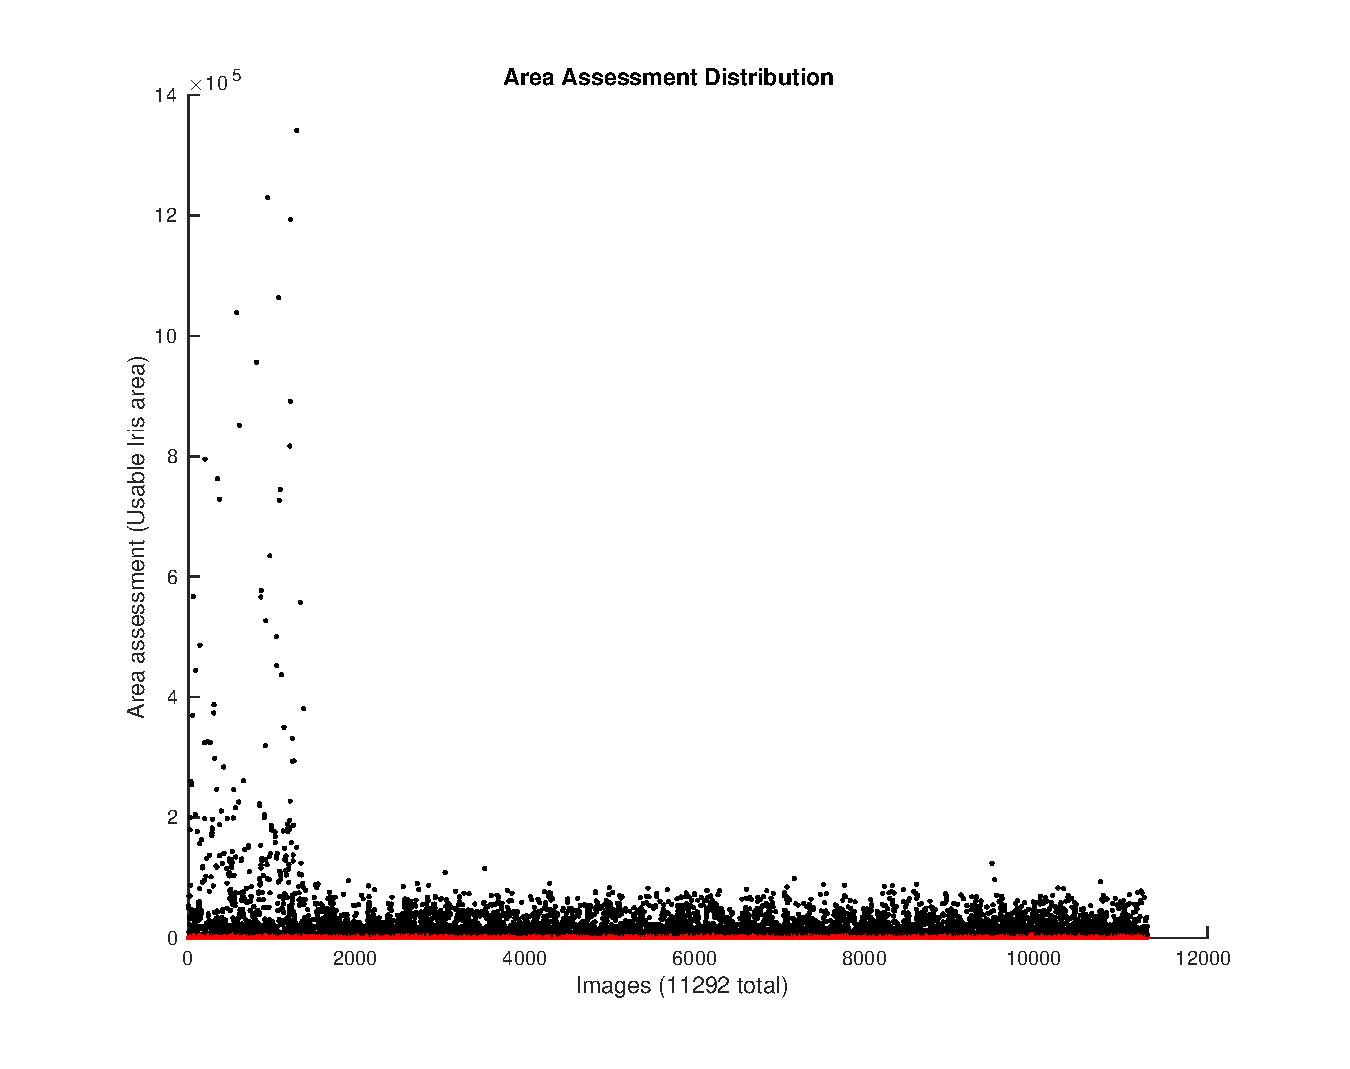
\includegraphics[width=0.9\linewidth, height=1.6cm]{pics/dist_area_assess}
		\caption{Dist. of the usable area\cite{hugo}}
		\label{fig:area}
	\end{minipage}
	\hfill
	\begin{minipage}{0.48\linewidth}
		\centering
		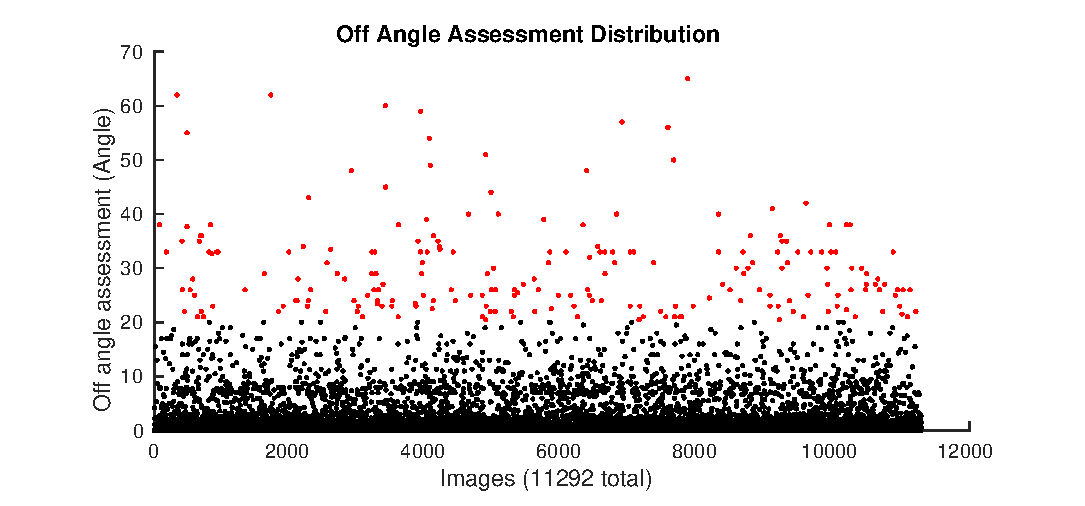
\includegraphics[width=0.9\linewidth, height=1.6cm]{pics/dist_off_angle_deg_2}
		\caption{Dist. of the off-angle \cite{hugo}}
		\label{fig:ang}
	\end{minipage}
	\begin{minipage}{0.48\linewidth}
		\centering
		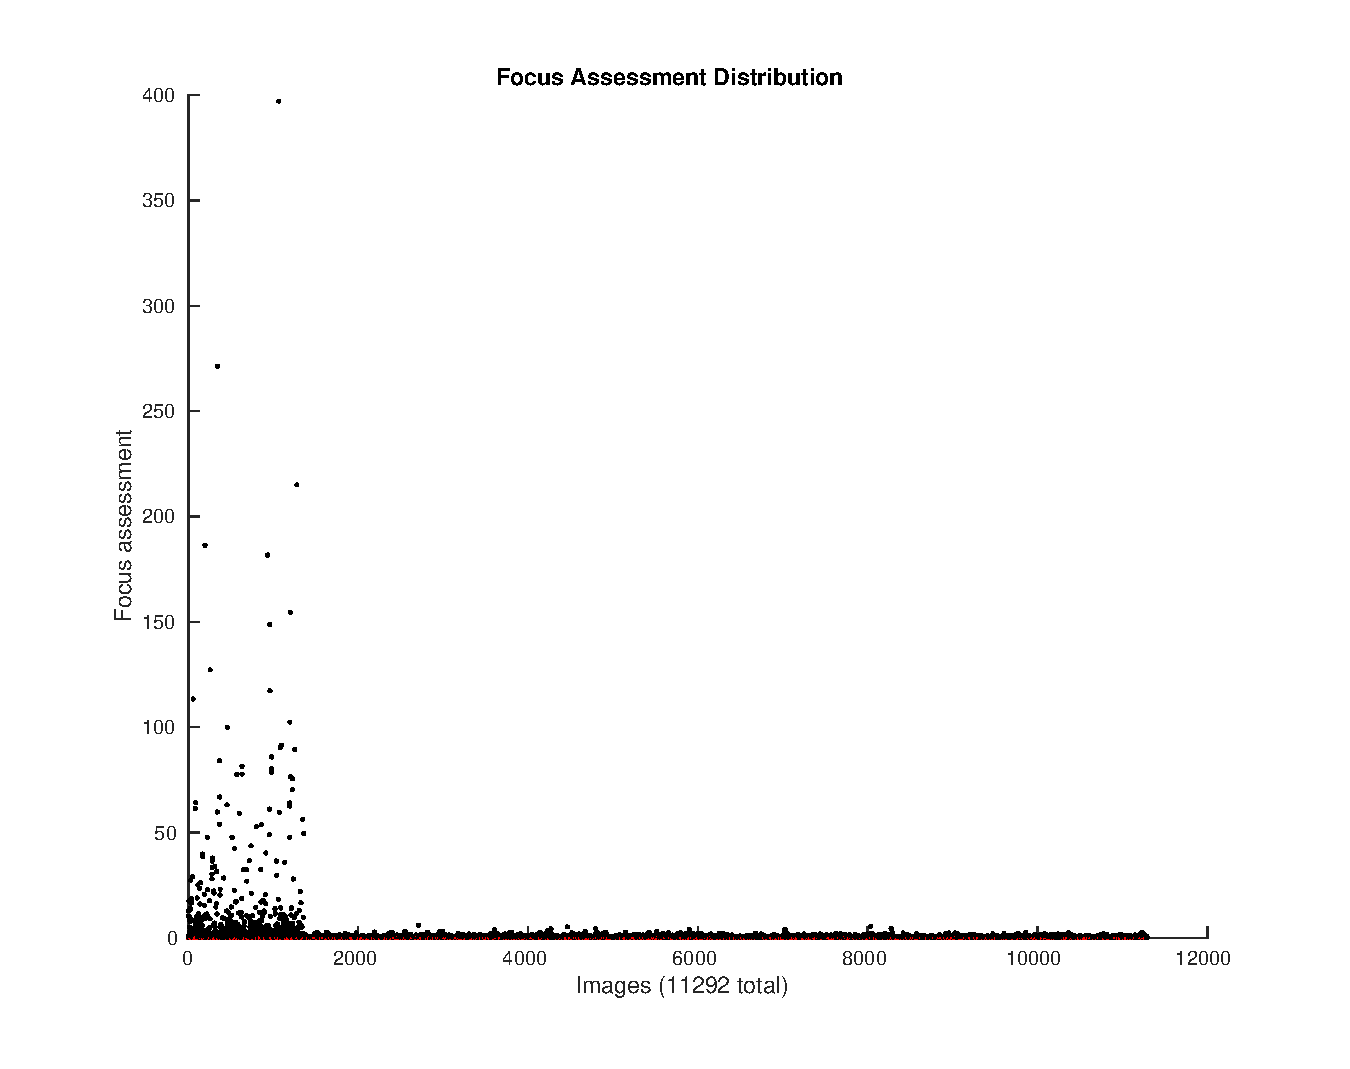
\includegraphics[width=0.9\linewidth, height=1.6cm]{pics/dist_focus_assess}
		\caption{Dist. of the focus assessment \cite{hugo}}
		\label{fig:focus} 
	\end{minipage}
	\hfill
	\begin{minipage}{0.48\linewidth}
		\centering
		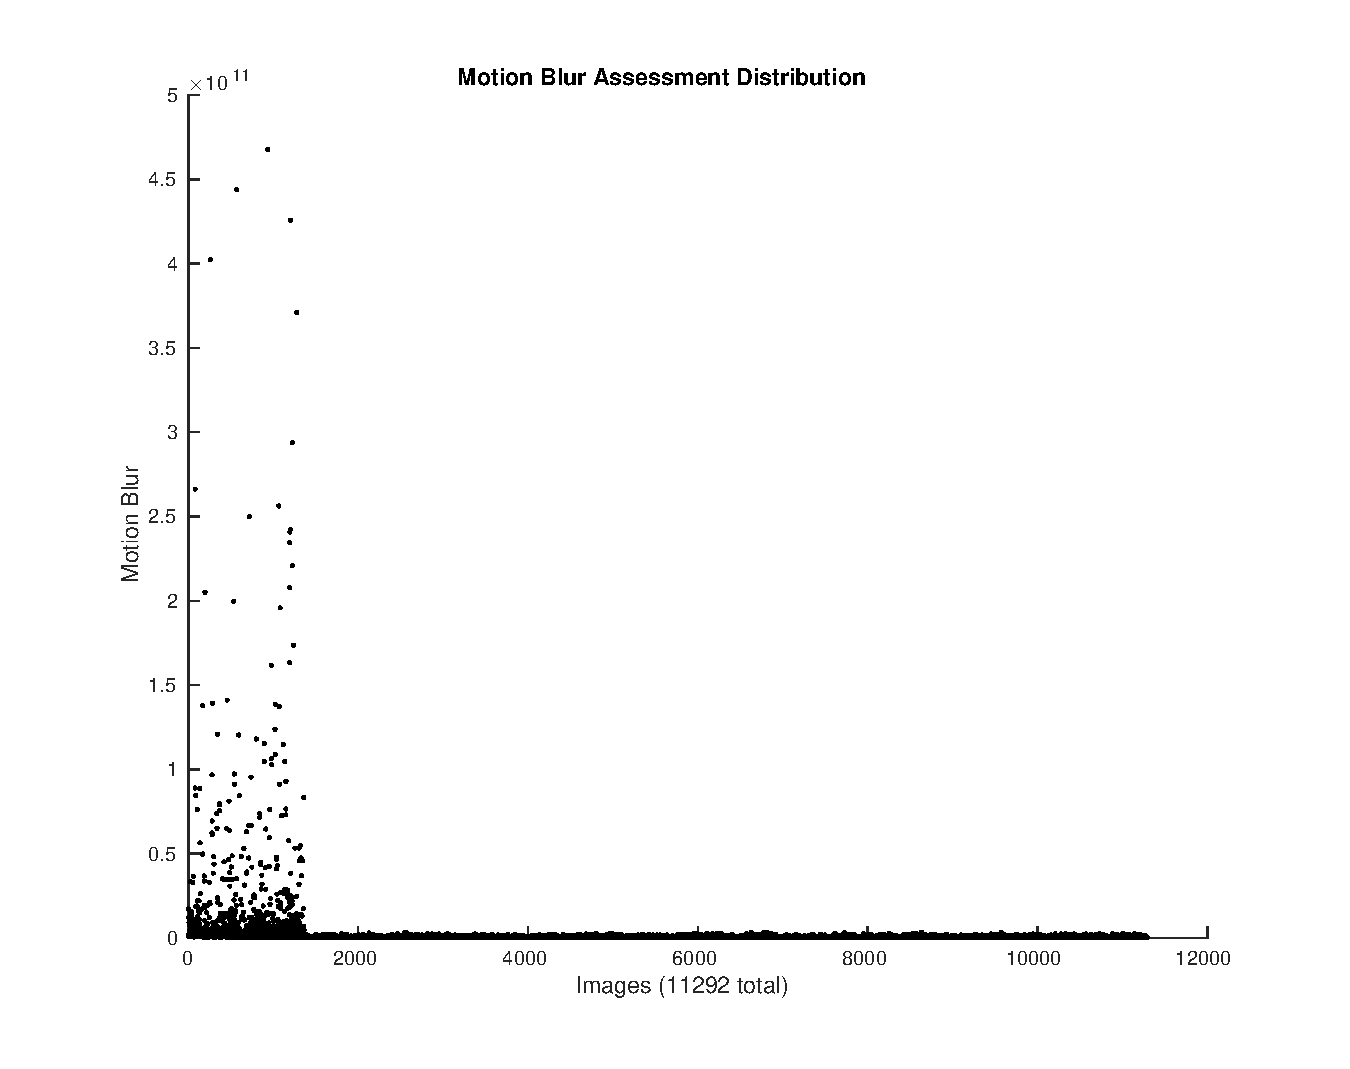
\includegraphics[width=0.9\linewidth, height=1.6cm]{pics/dist_motion_blur_mag}
		\caption{Dist. of the motion blur mag. \cite{hugo}}
		\label{fig:motion}
	\end{minipage}
	\begin{minipage}{0.48\linewidth}
		\centering
		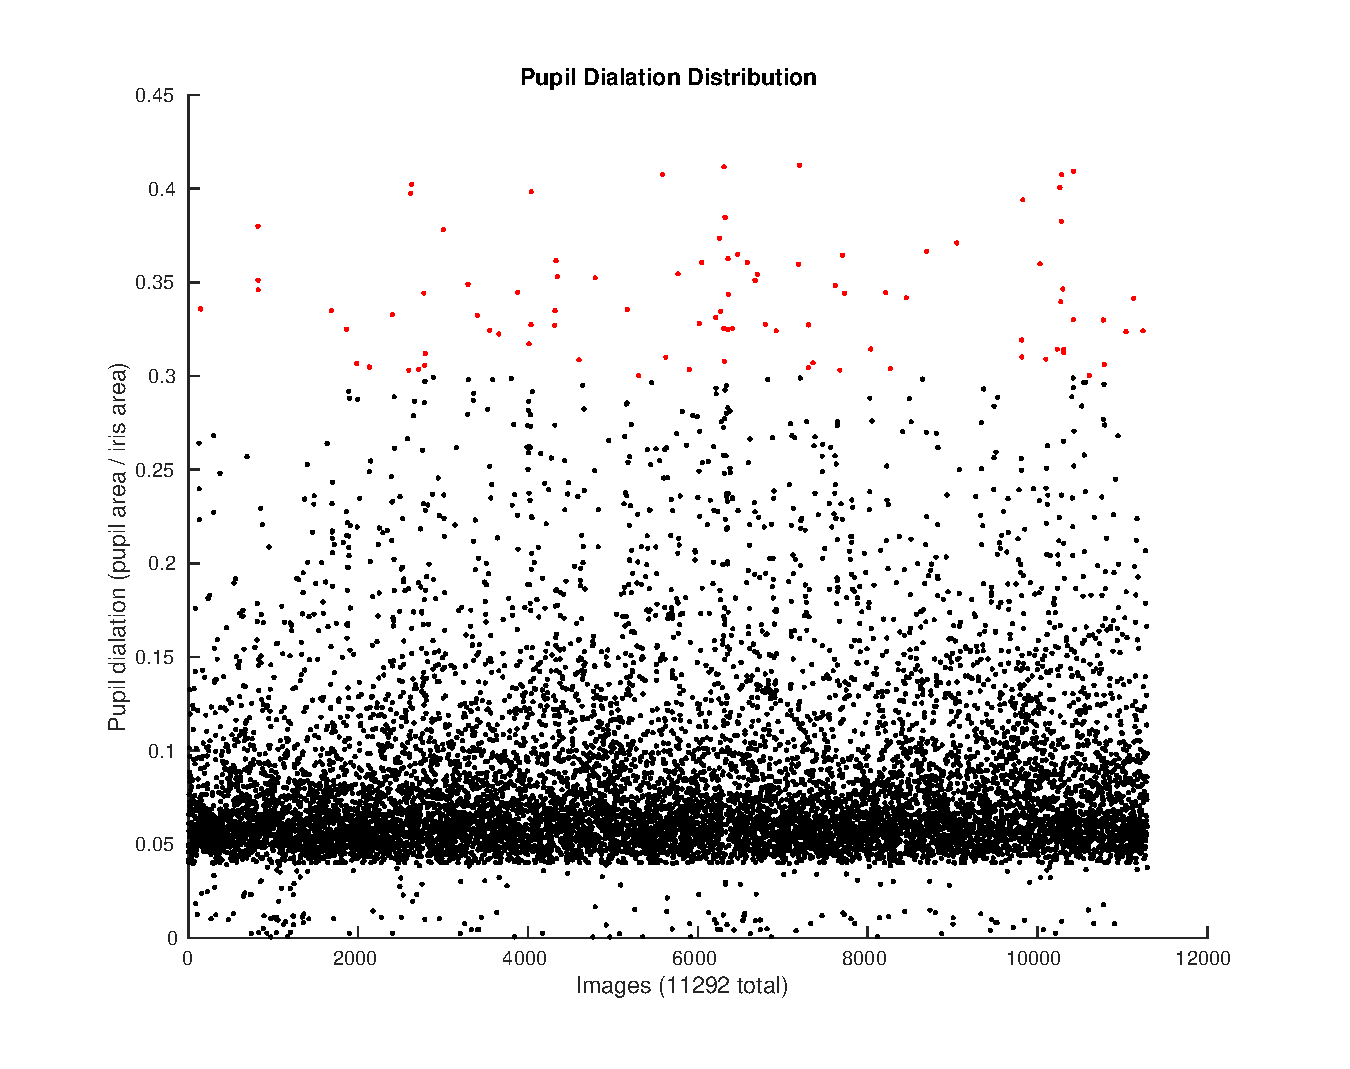
\includegraphics[width=0.9\linewidth, height=1.6cm]{pics/dist_pupil_dilation_ratio}
		\caption{Dist. of the pupil/iris ratio \cite{hugo}}
		\label{fig:ratio}
	\end{minipage}
	\hfill
	\begin{minipage}{0.48\linewidth}
		\centering
		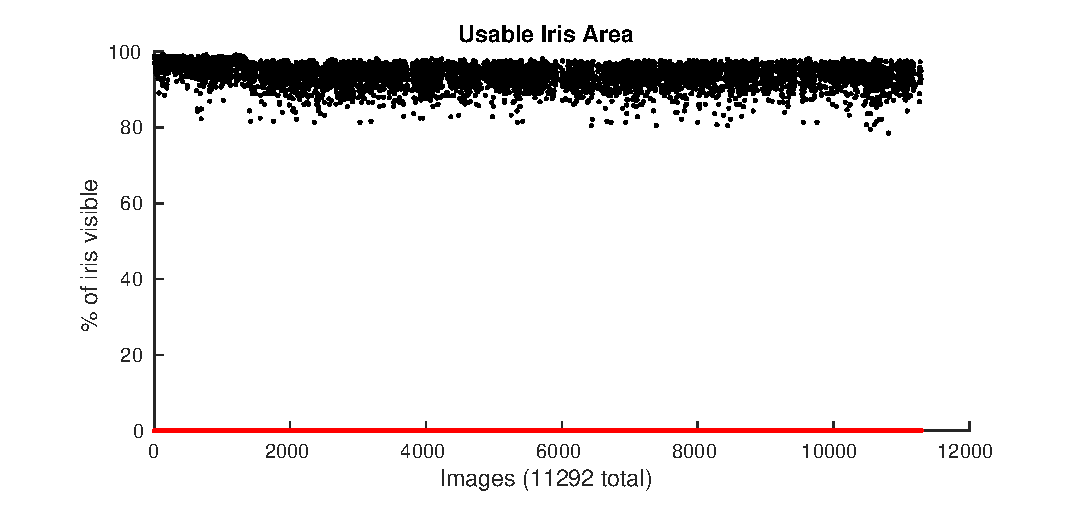
\includegraphics[width=0.9\linewidth, height=1.6cm]{pics/biqa_dist_uia}
		\caption{Dist. of the usable iris area \cite{iso}}
		\label{fig:uia}
	\end{minipage}
	\begin{minipage}{0.48\linewidth}
		\centering
		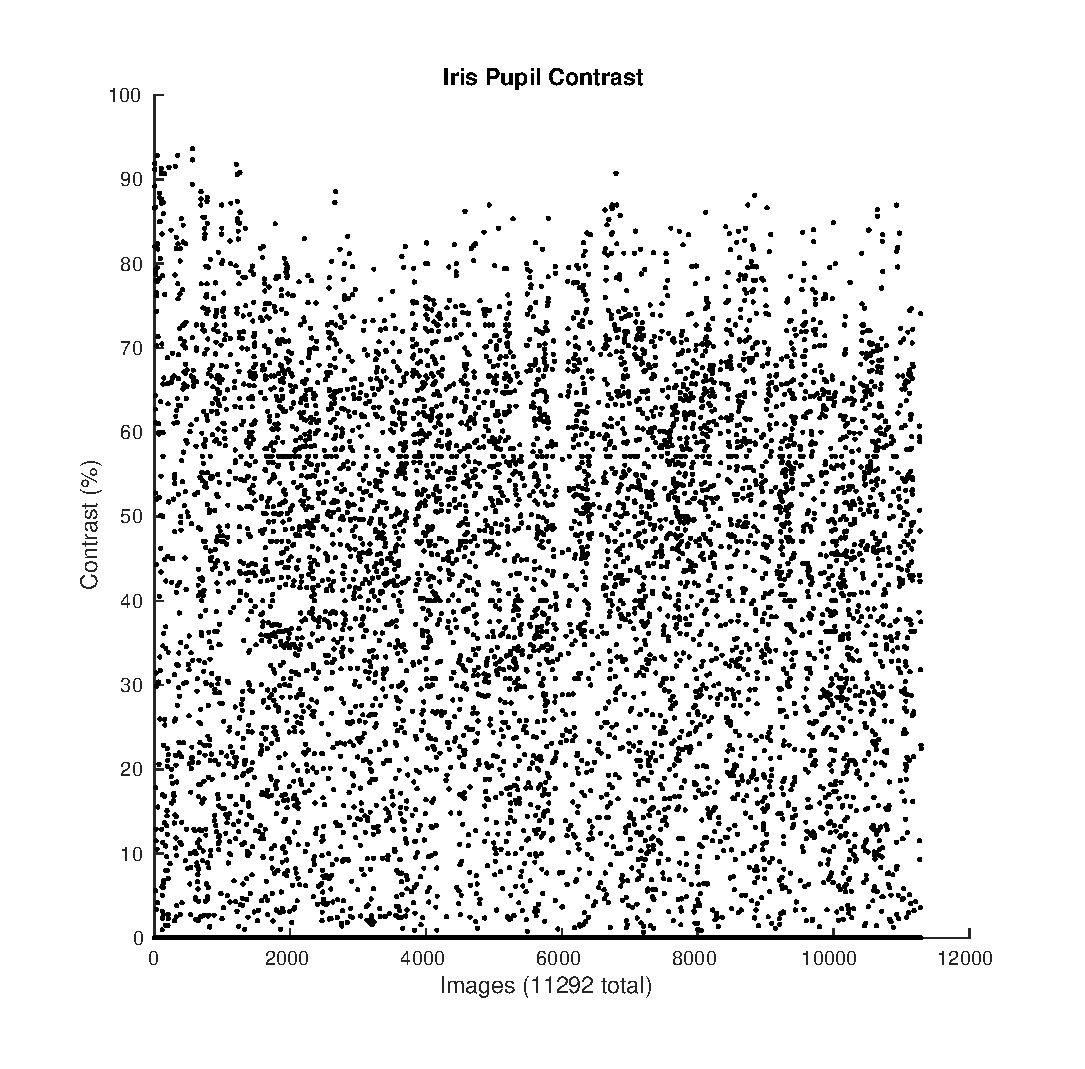
\includegraphics[width=0.9\linewidth, height=1.6cm]{pics/biqa_dist_ipc}
		\caption{Dist. of the pupil-iris contrast \cite{iso}}
		\label{fig:ipc}
	\end{minipage}
	\hfill
	\begin{minipage}{0.48\linewidth}
		\centering
		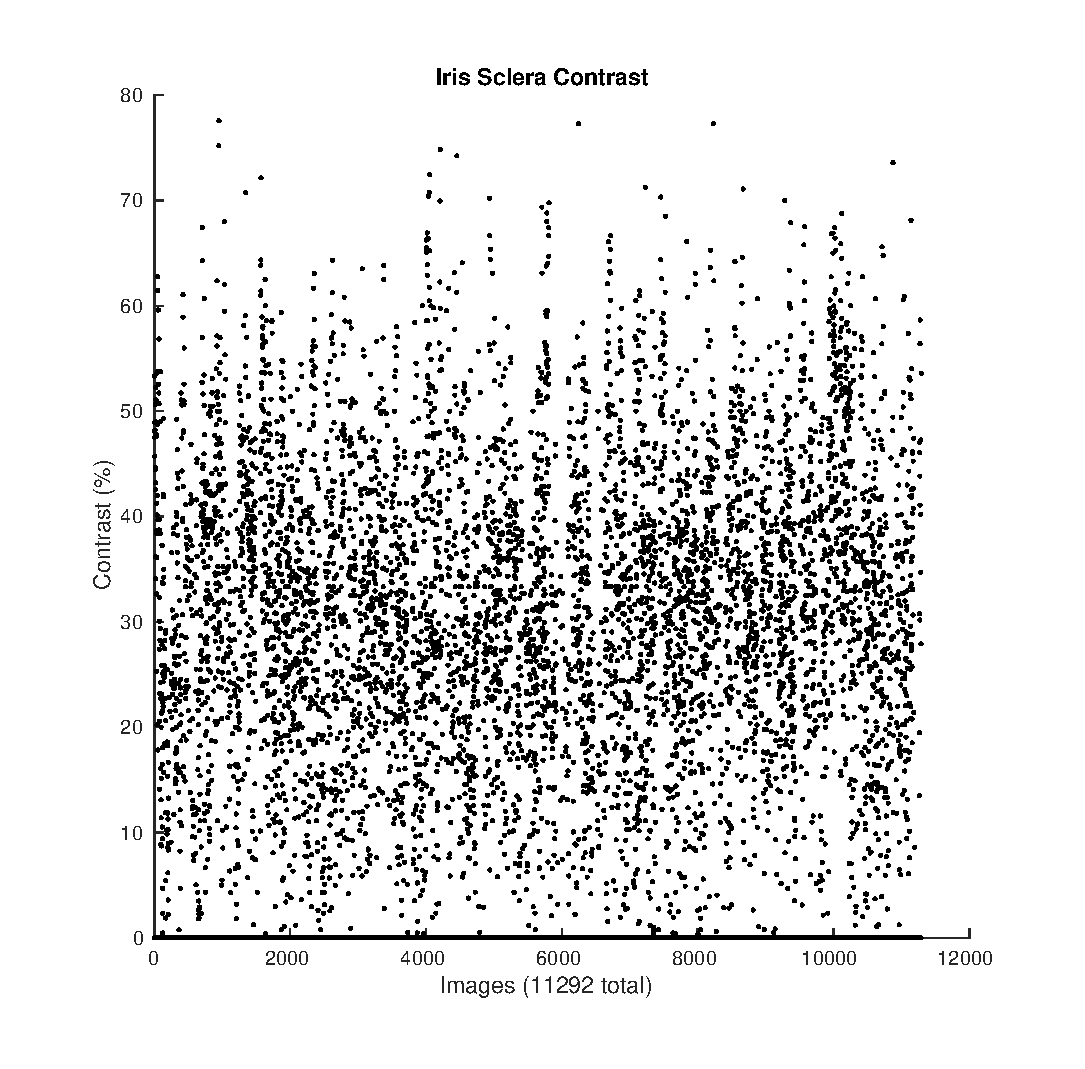
\includegraphics[width=0.9\linewidth, height=1.6cm]{pics/biqa_dist_isc}
		\caption{Dist. of the iris-sclera \cite{iso}}
		\label{fig:isc}
	\end{minipage}
	\begin{minipage}{0.48\linewidth}
		\centering
		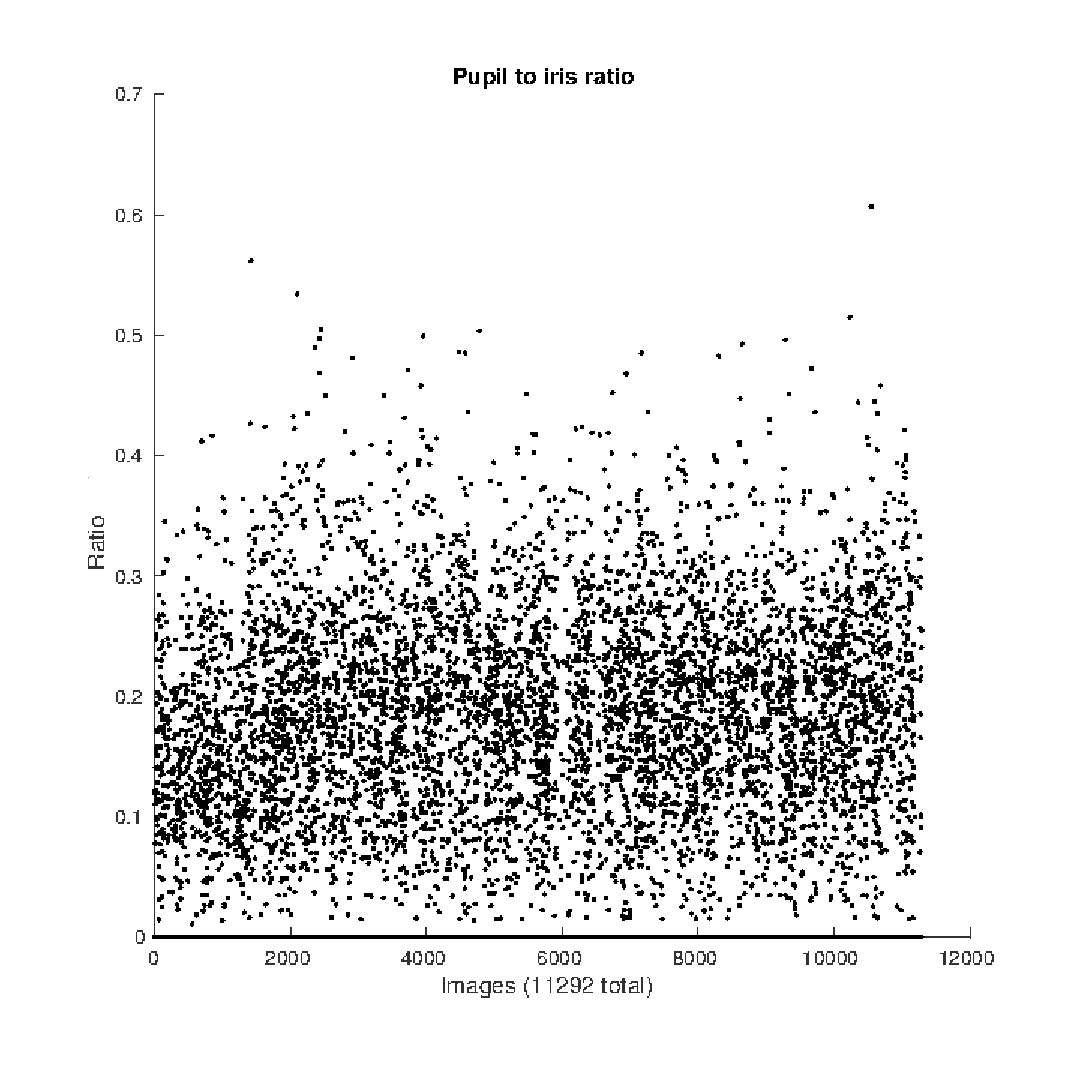
\includegraphics[width=0.9\linewidth, height=1.6cm]{pics/biqa_dist_pup_ir_ratio}
		\caption{Dist. of the pupil-iris ratio \cite{iso}}
		\label{fig:pir}
	\end{minipage}
	\hfill
	\begin{minipage}{0.48\linewidth}
		\centering
		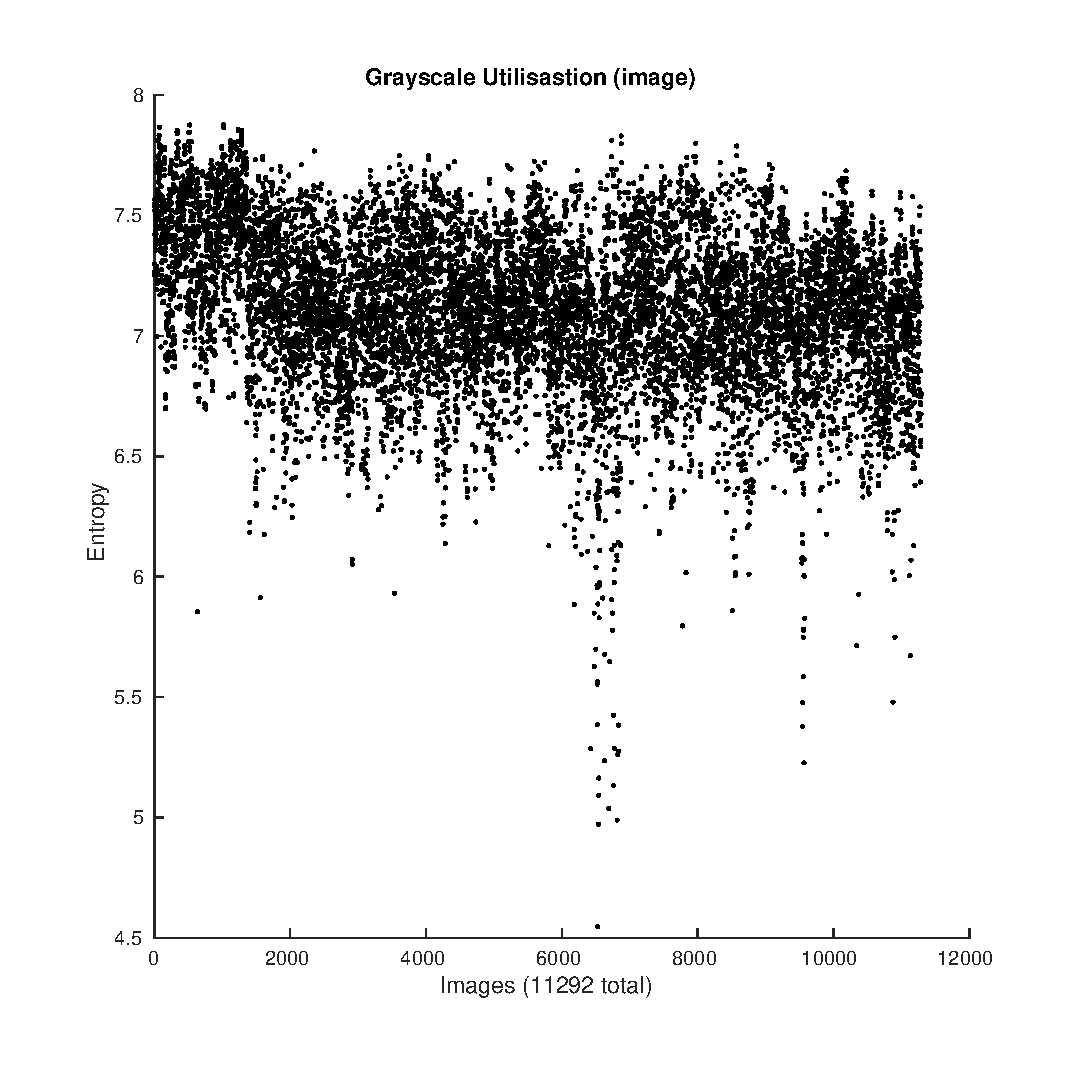
\includegraphics[width=0.9\linewidth, height=1.6cm]{pics/biqa_dist_gsu_full}
		\caption{Dist. of the GSU for the image \cite{iso}}
		\label{fig:gsuf}
	\end{minipage}
	\begin{minipage}{0.48\linewidth}
		\centering
		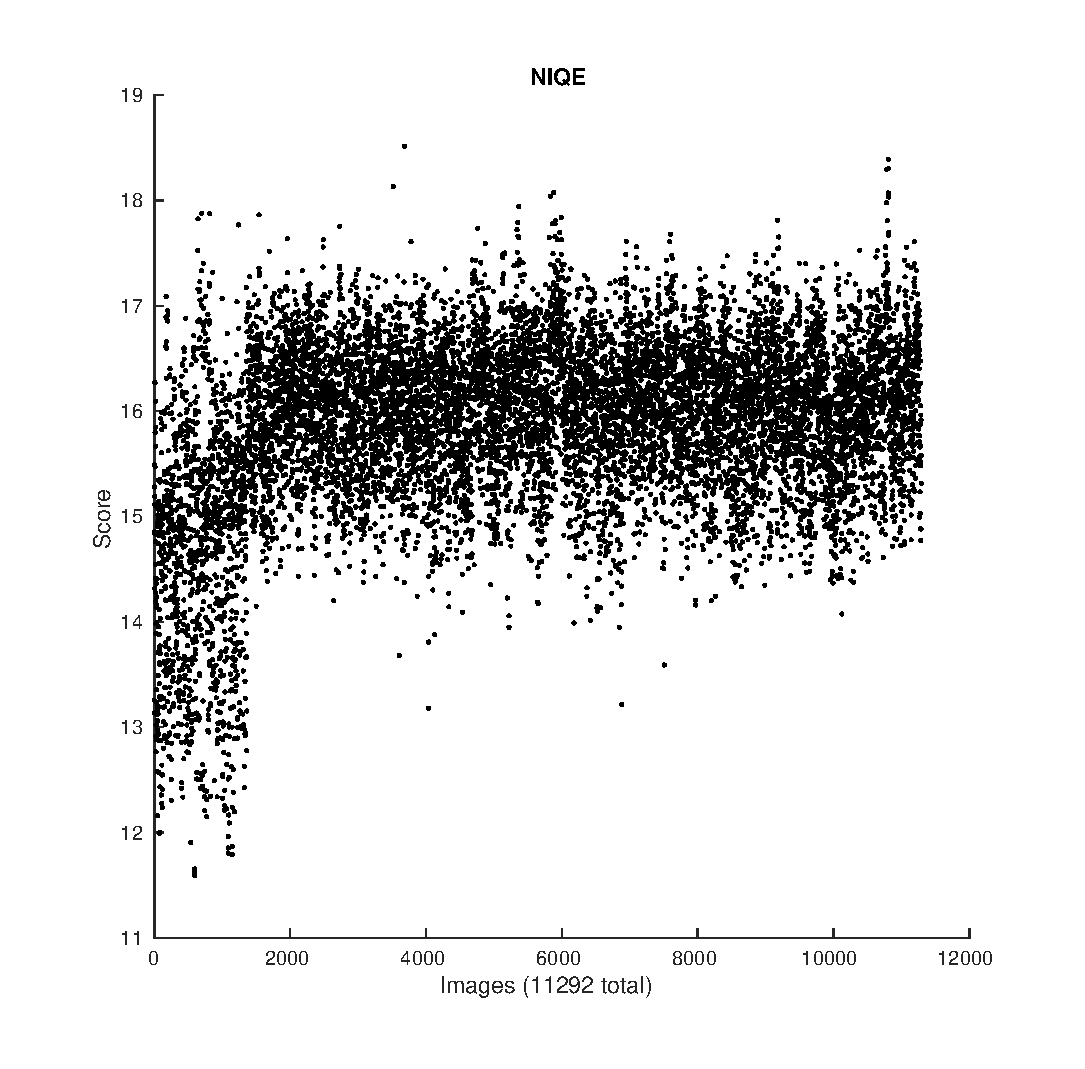
\includegraphics[width=0.9\linewidth, height=1.6cm]{pics/biqa_dist_niqe}
		\caption{Dist. of the NIQE \cite{niqe}}
		\label{fig:niqe}
	\end{minipage}
	\hfill
	\begin{minipage}{0.48\linewidth}
		\centering
		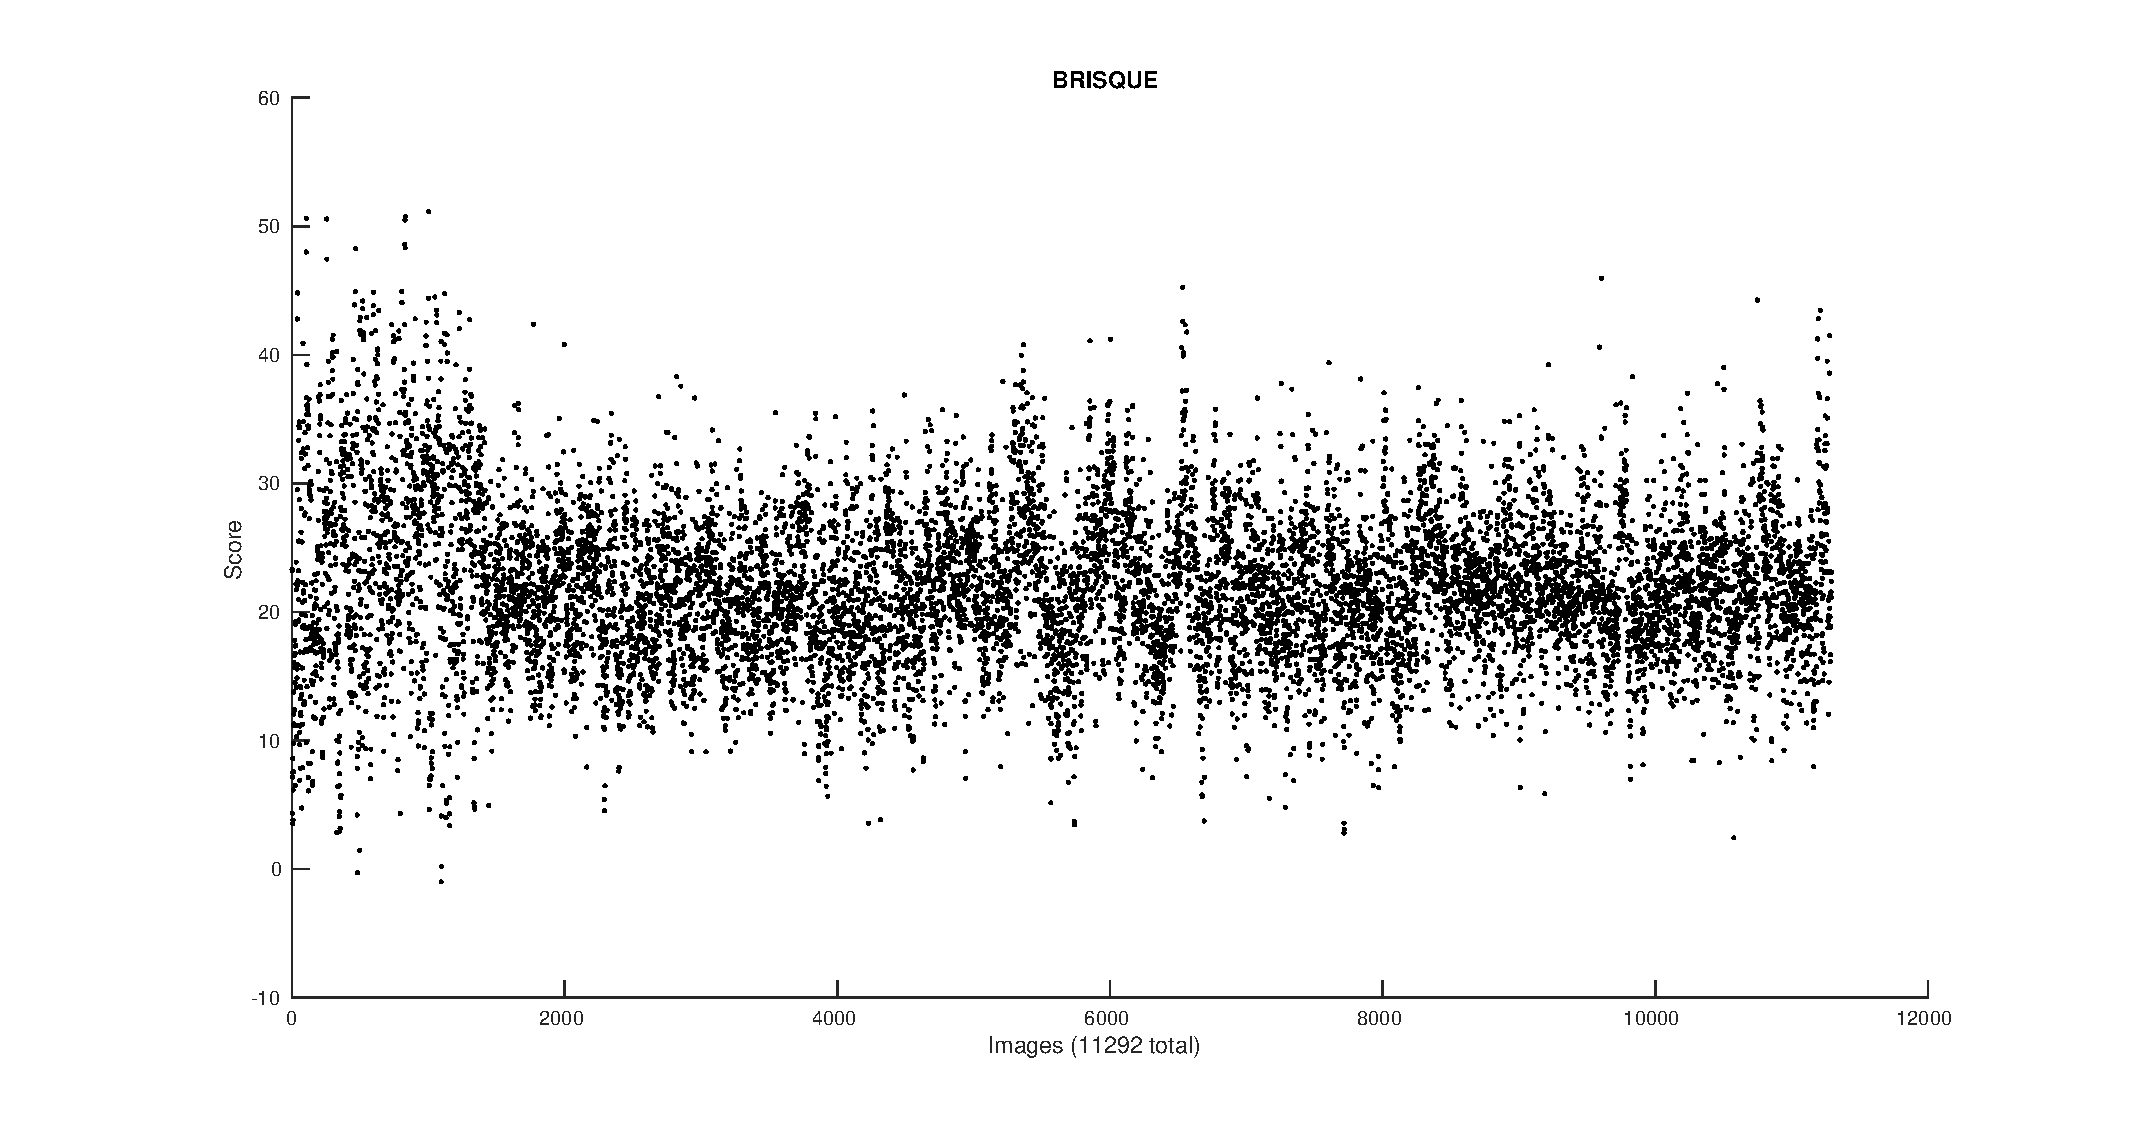
\includegraphics[width=0.9\linewidth, height=1.6cm]{pics/biqa_dist_brisque}
		\caption{Dist. of the BRISQUE \cite{brisque}}
		\label{fig:brisque}
	\end{minipage}
	\begin{minipage}{0.48\linewidth}
		\centering
		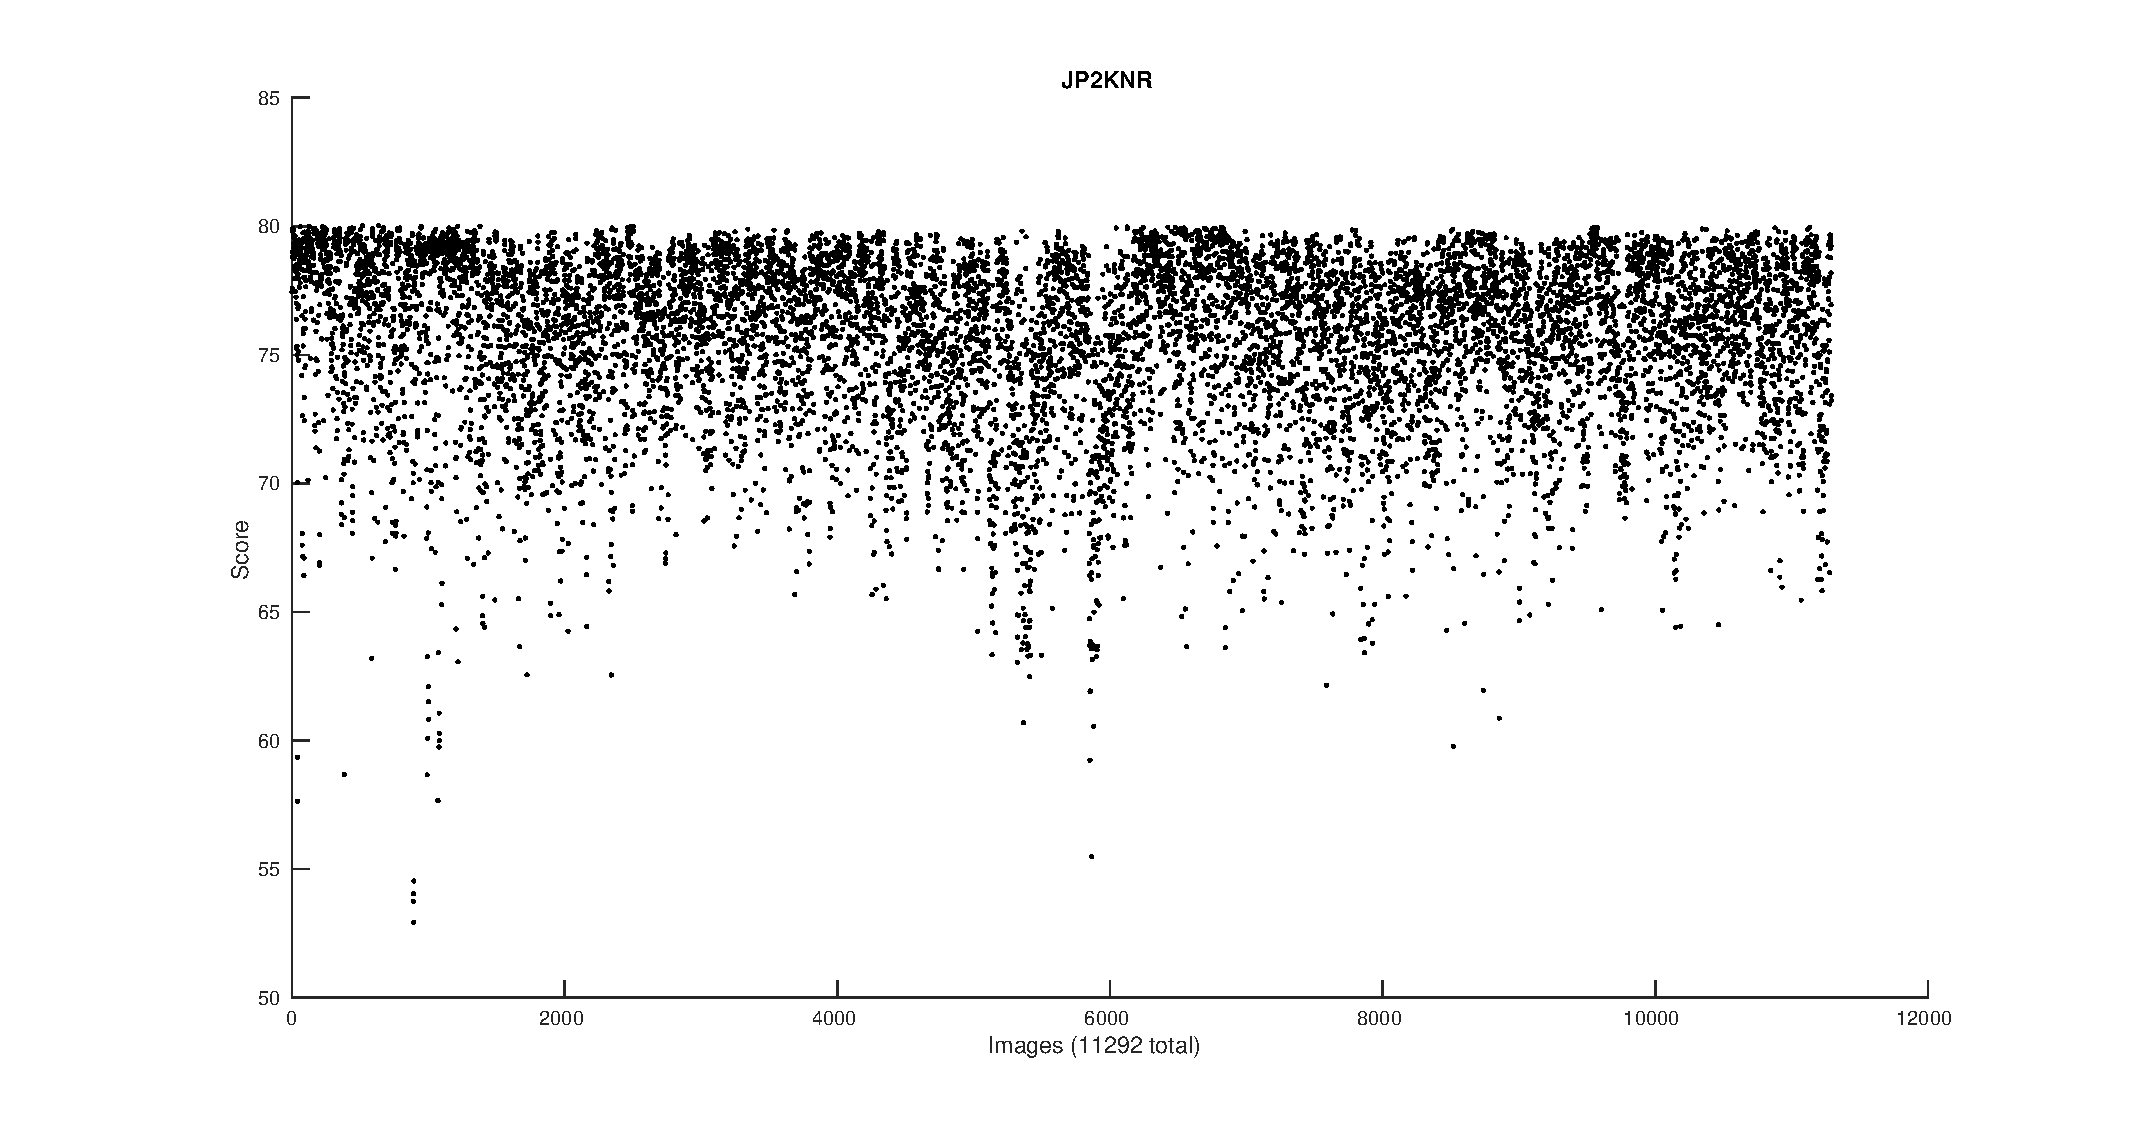
\includegraphics[width=0.9\linewidth, height=1.6cm]{pics/biqa_dist_jp2knr}
		\caption{Dist. of the JP2KNR \cite{jp2knr}}
		\label{fig:jp2knr}
	\end{minipage}
	\hfill
	\begin{minipage}{0.48\linewidth}
		\centering
		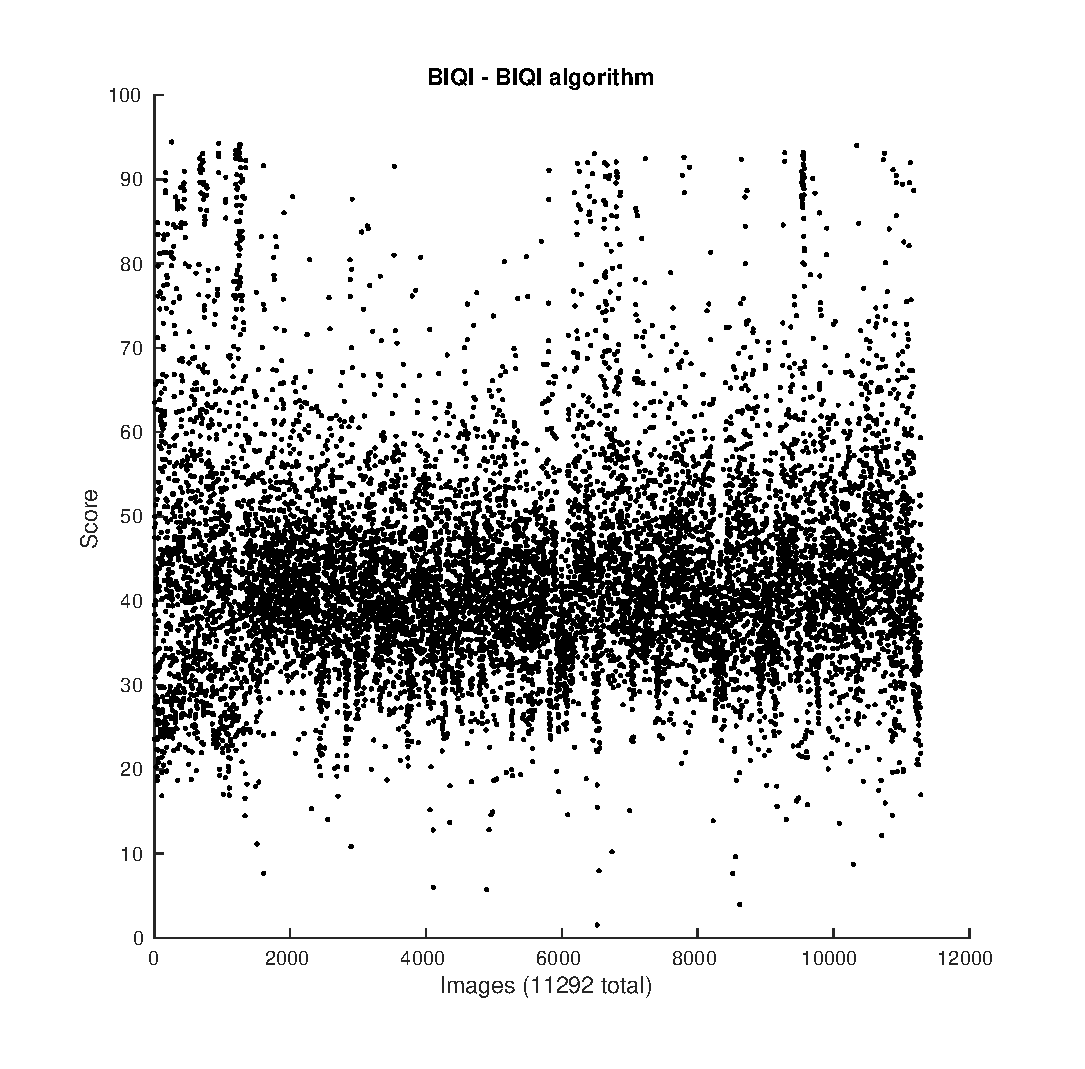
\includegraphics[width=0.9\linewidth, height=1.6cm]{pics/biqa_dist_biqi_alg}
		\caption{Dist. of the BIQI, algorithm \cite{biqi}}
		\label{fig:biqialg}
	\end{minipage}
\end{figure}
\begin{figure}
	\begin{minipage}{0.48\linewidth}
		\centering
		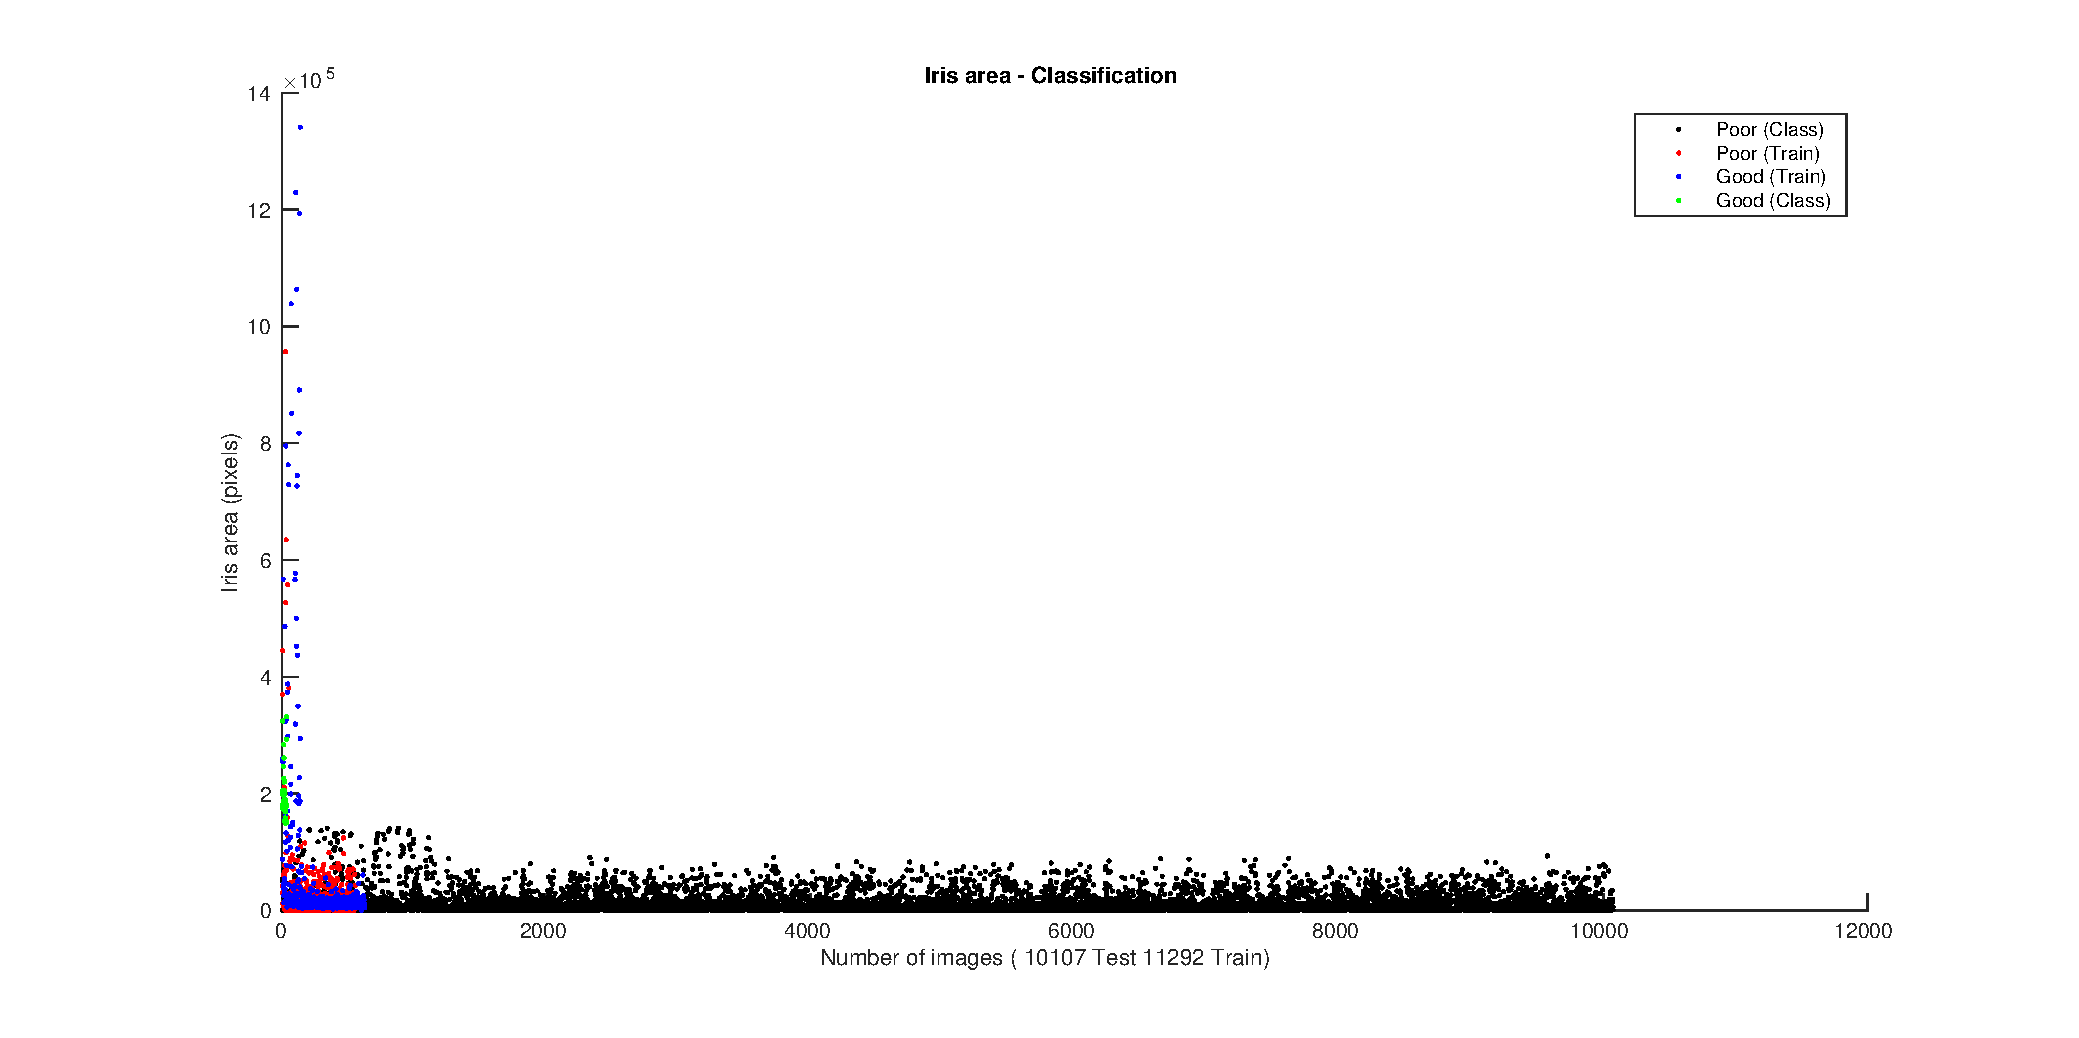
\includegraphics[width=0.9\linewidth, height=1.6cm]{pics/iqa_clas_area}
		\caption{Res. of class. using IQA iris area}
		\label{fig:clas_ia}
	\end{minipage}
	\hfill
	\begin{minipage}{0.48\linewidth}
		\centering
		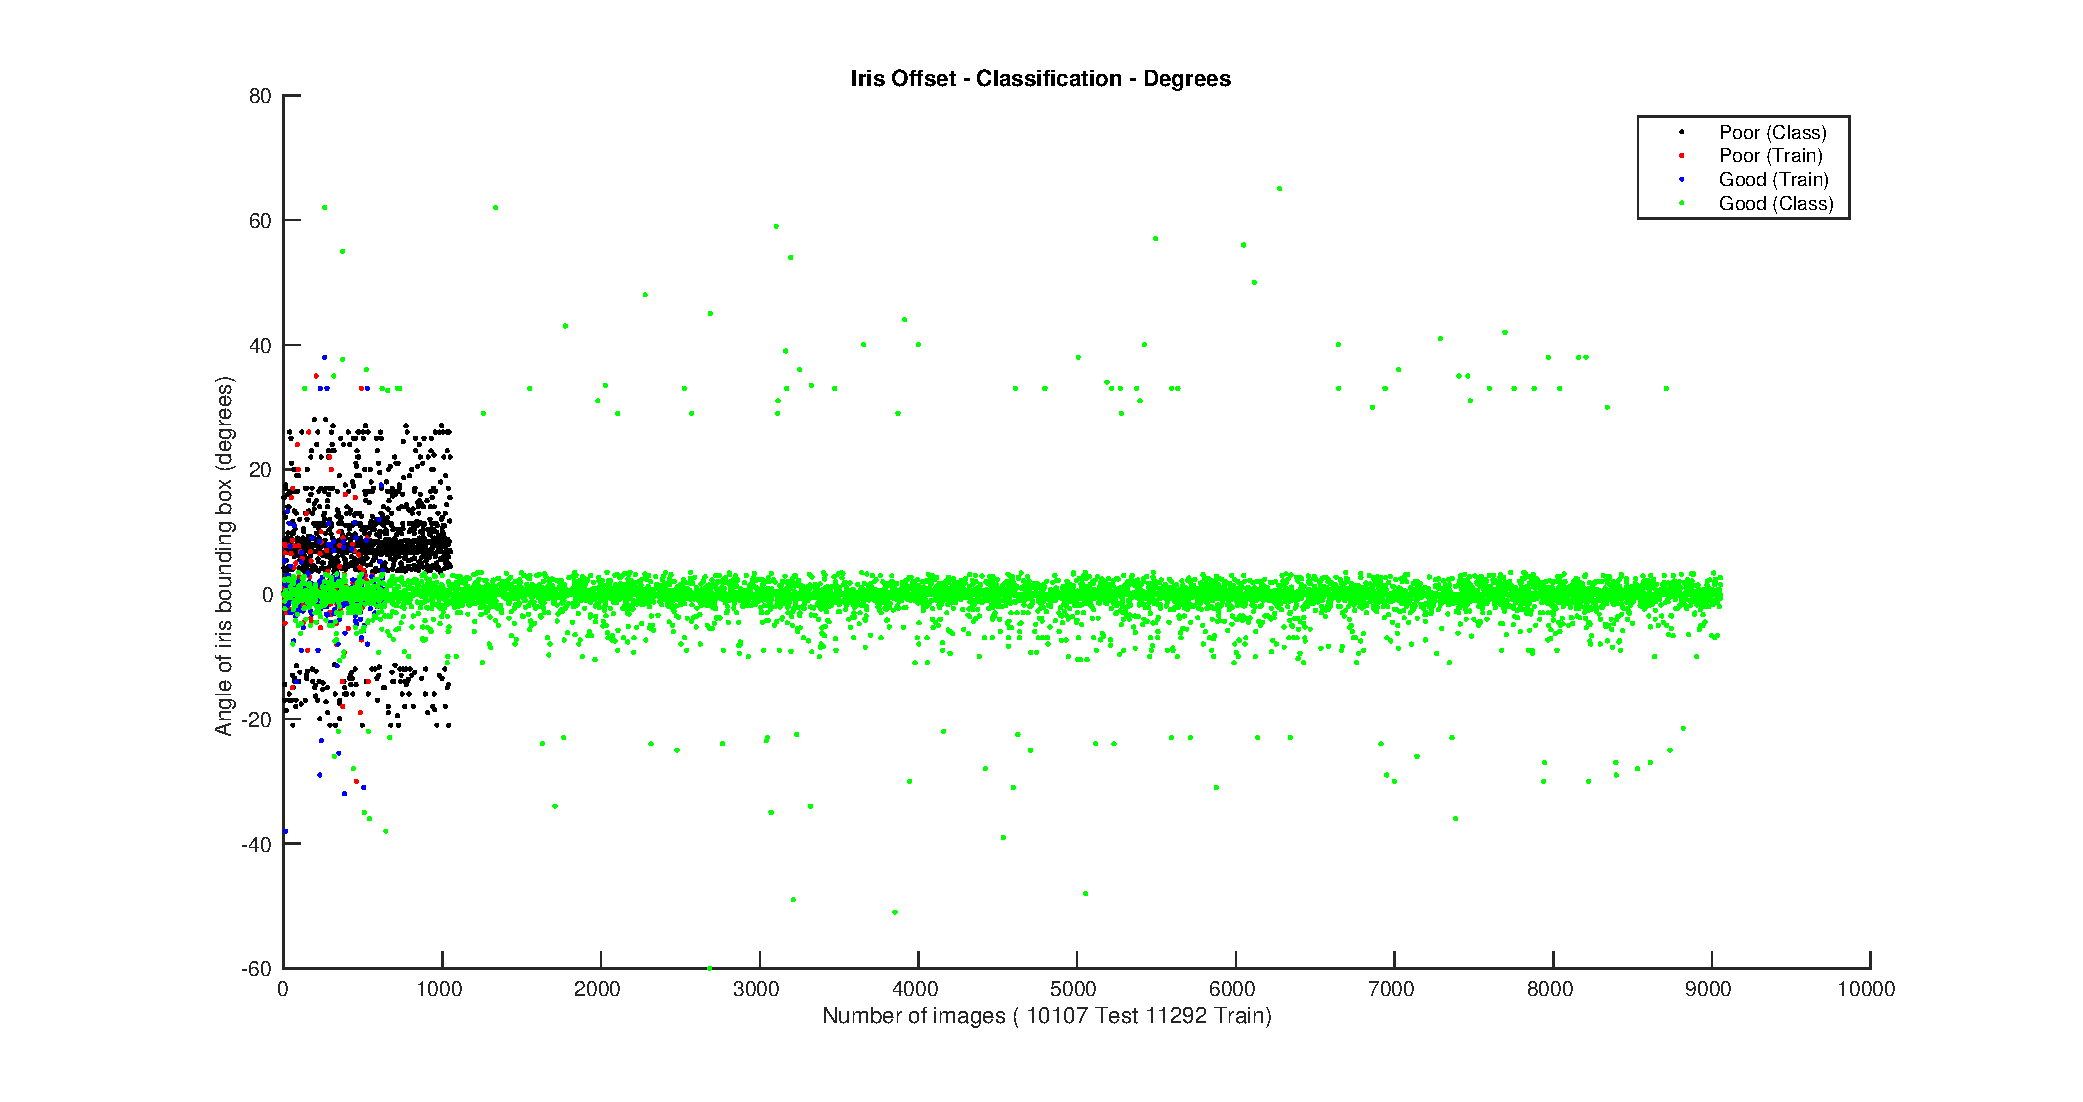
\includegraphics[width=0.9\linewidth, height=1.6cm]{pics/iqa_clas_iris_angle}
		\caption{Res. of class. using IQA iris angle}
		\label{fig:clas_ang}
	\end{minipage}
	\begin{minipage}{0.48\linewidth}
		\centering
		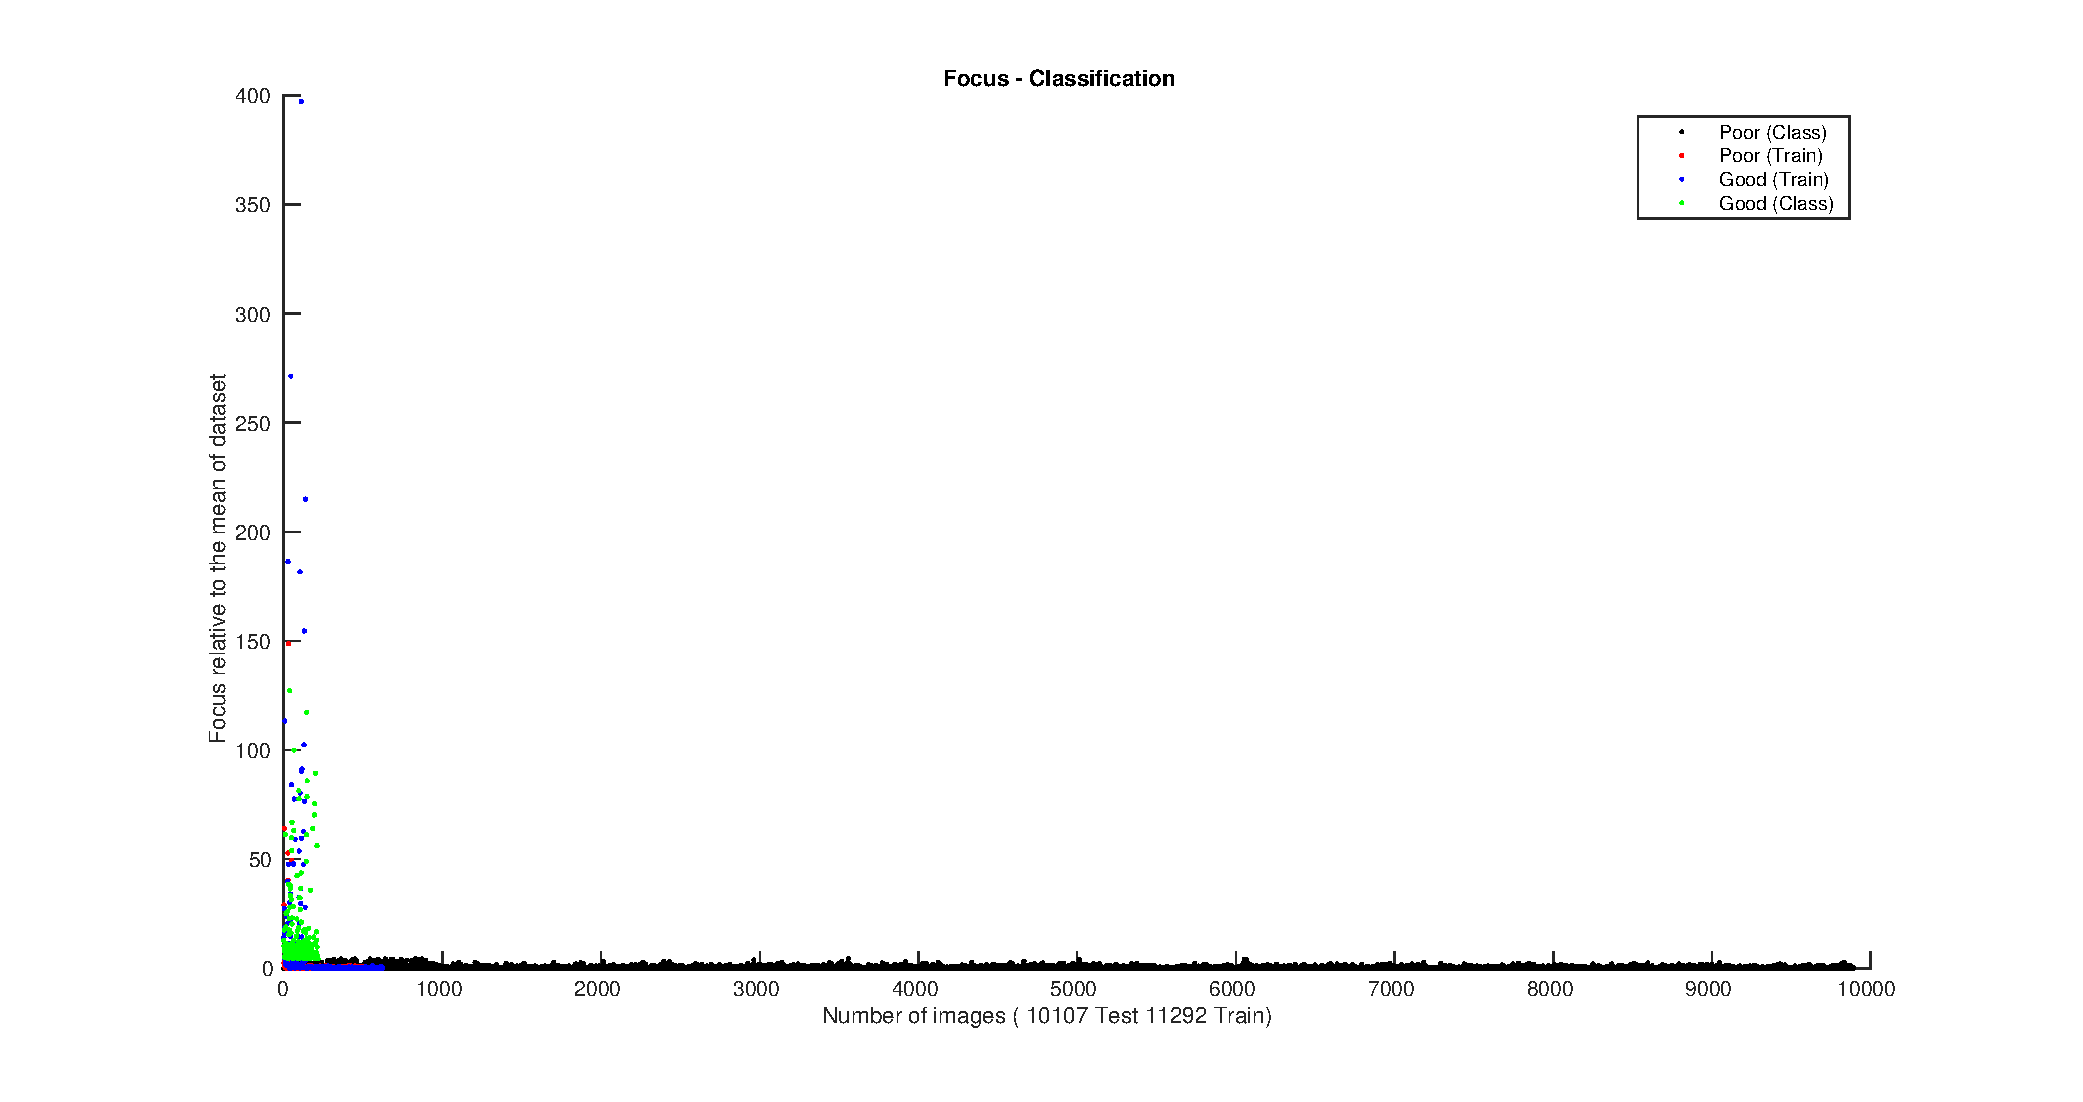
\includegraphics[width=0.9\linewidth, height=1.6cm]{pics/iqa_clas_focus}
		\caption{Res. of class. using IQA focus}
		\label{fig:clas_f}
	\end{minipage}
	\hfill
	\begin{minipage}{0.48\linewidth}
		\centering
		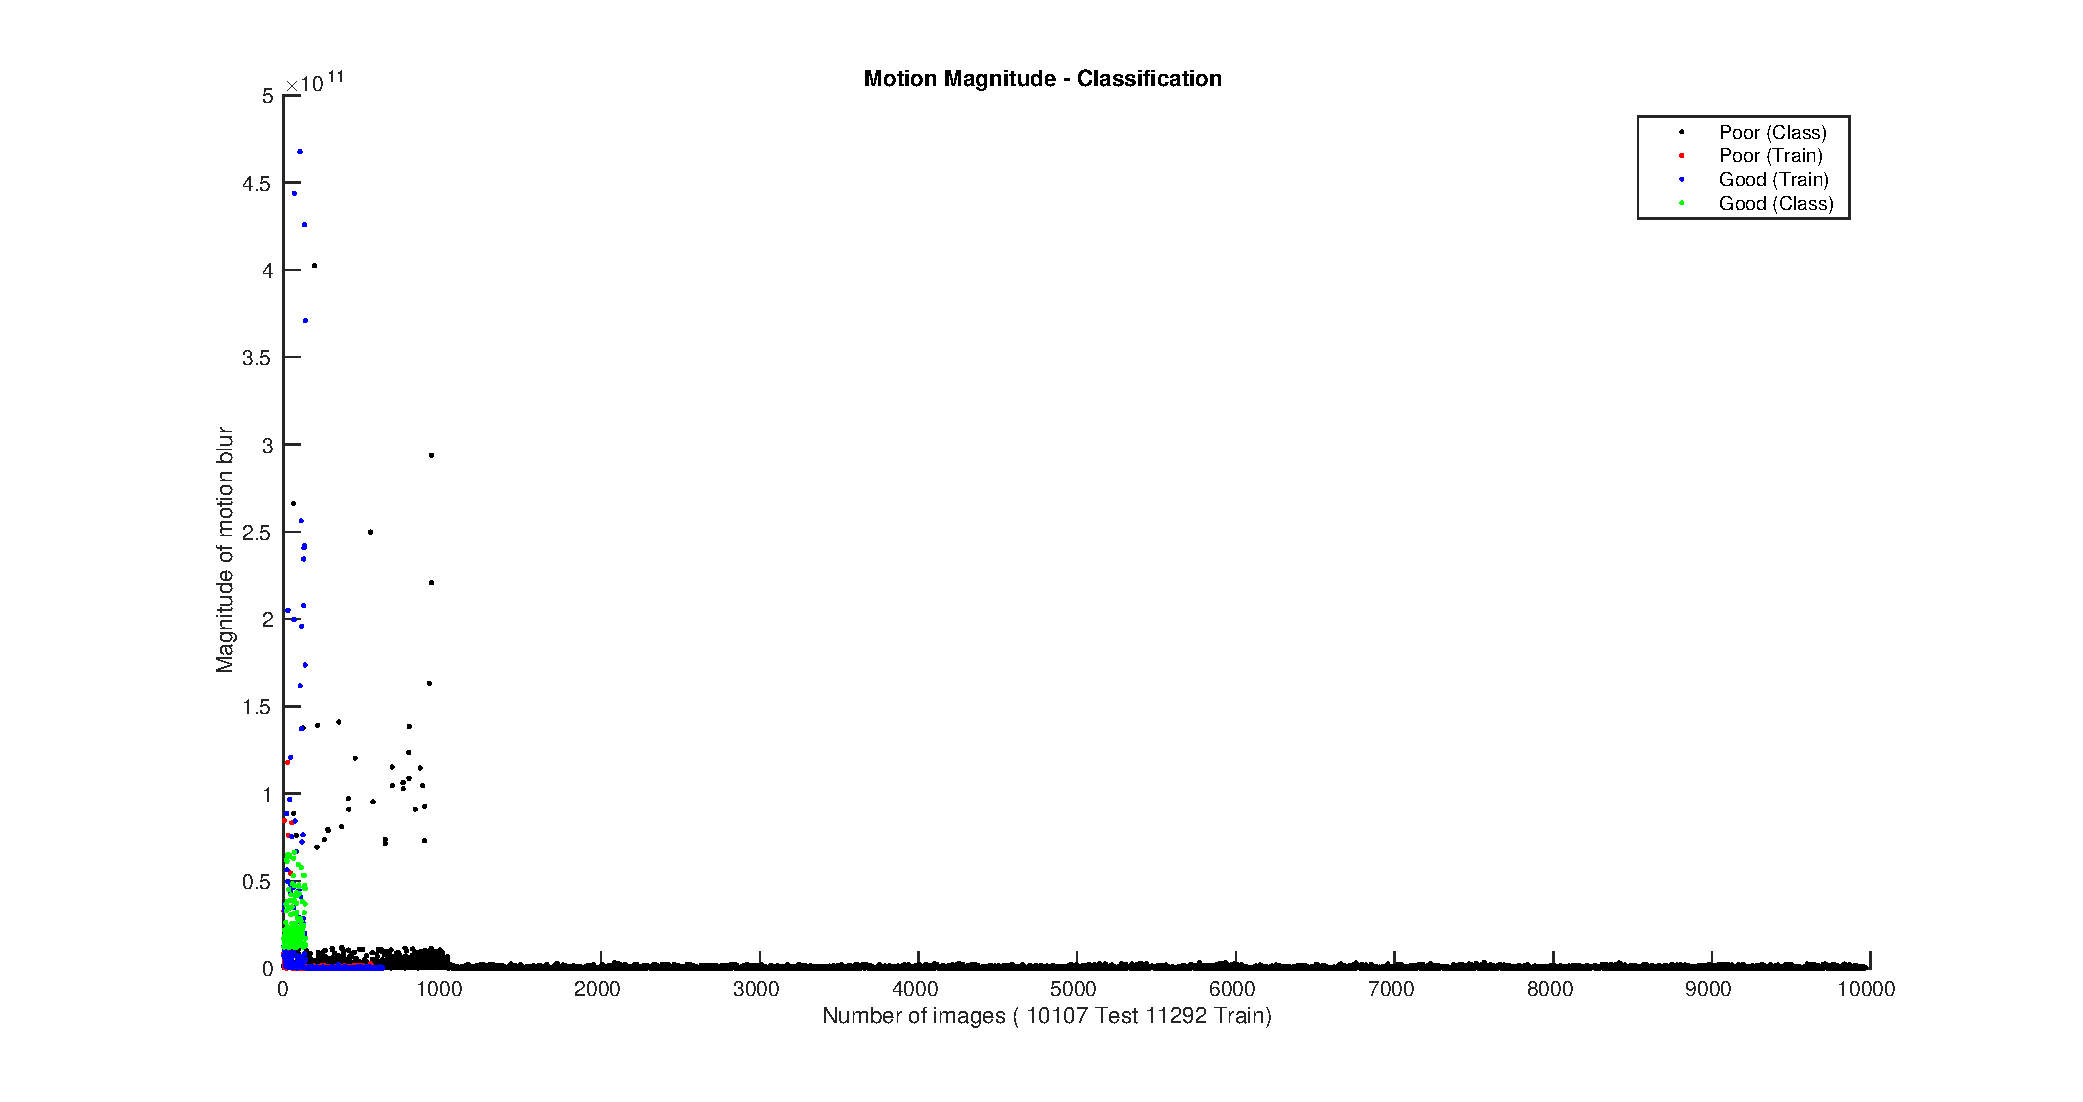
\includegraphics[width=0.9\linewidth, height=1.6cm]{pics/iqa_clas_motion}
		\caption{Res. of class. using IQA motion}
		\label{fig:clas_mot}
	\end{minipage}
	\begin{minipage}{0.48\linewidth}
		\centering
		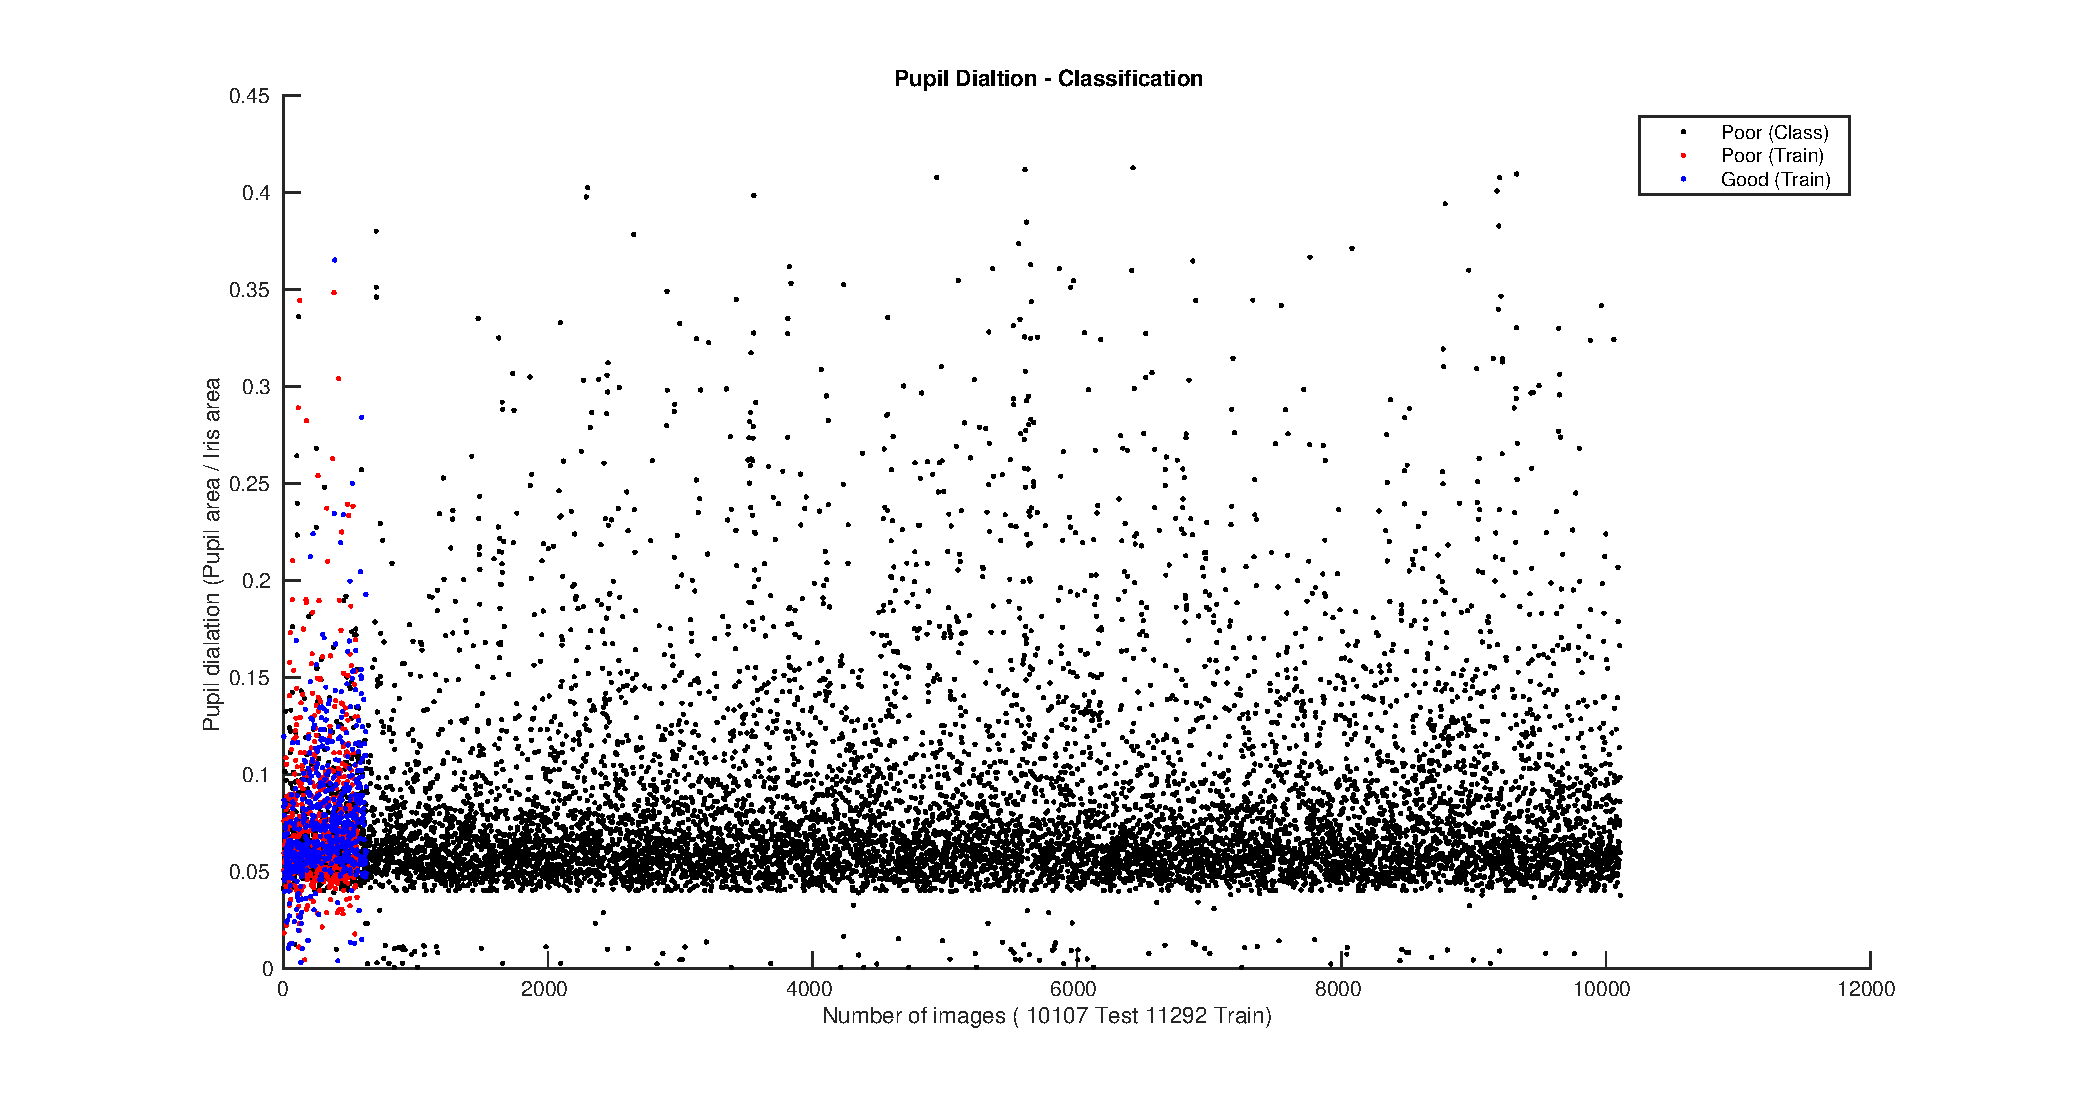
\includegraphics[width=0.9\linewidth, height=1.6cm]{pics/iqa_clas_pup_dial}
		\caption{Res. of class. using IQA pupil dilation}
		\label{fig:clas_pd}
	\end{minipage}
	\hfill
	\begin{minipage}{0.48\linewidth}
		\centering
		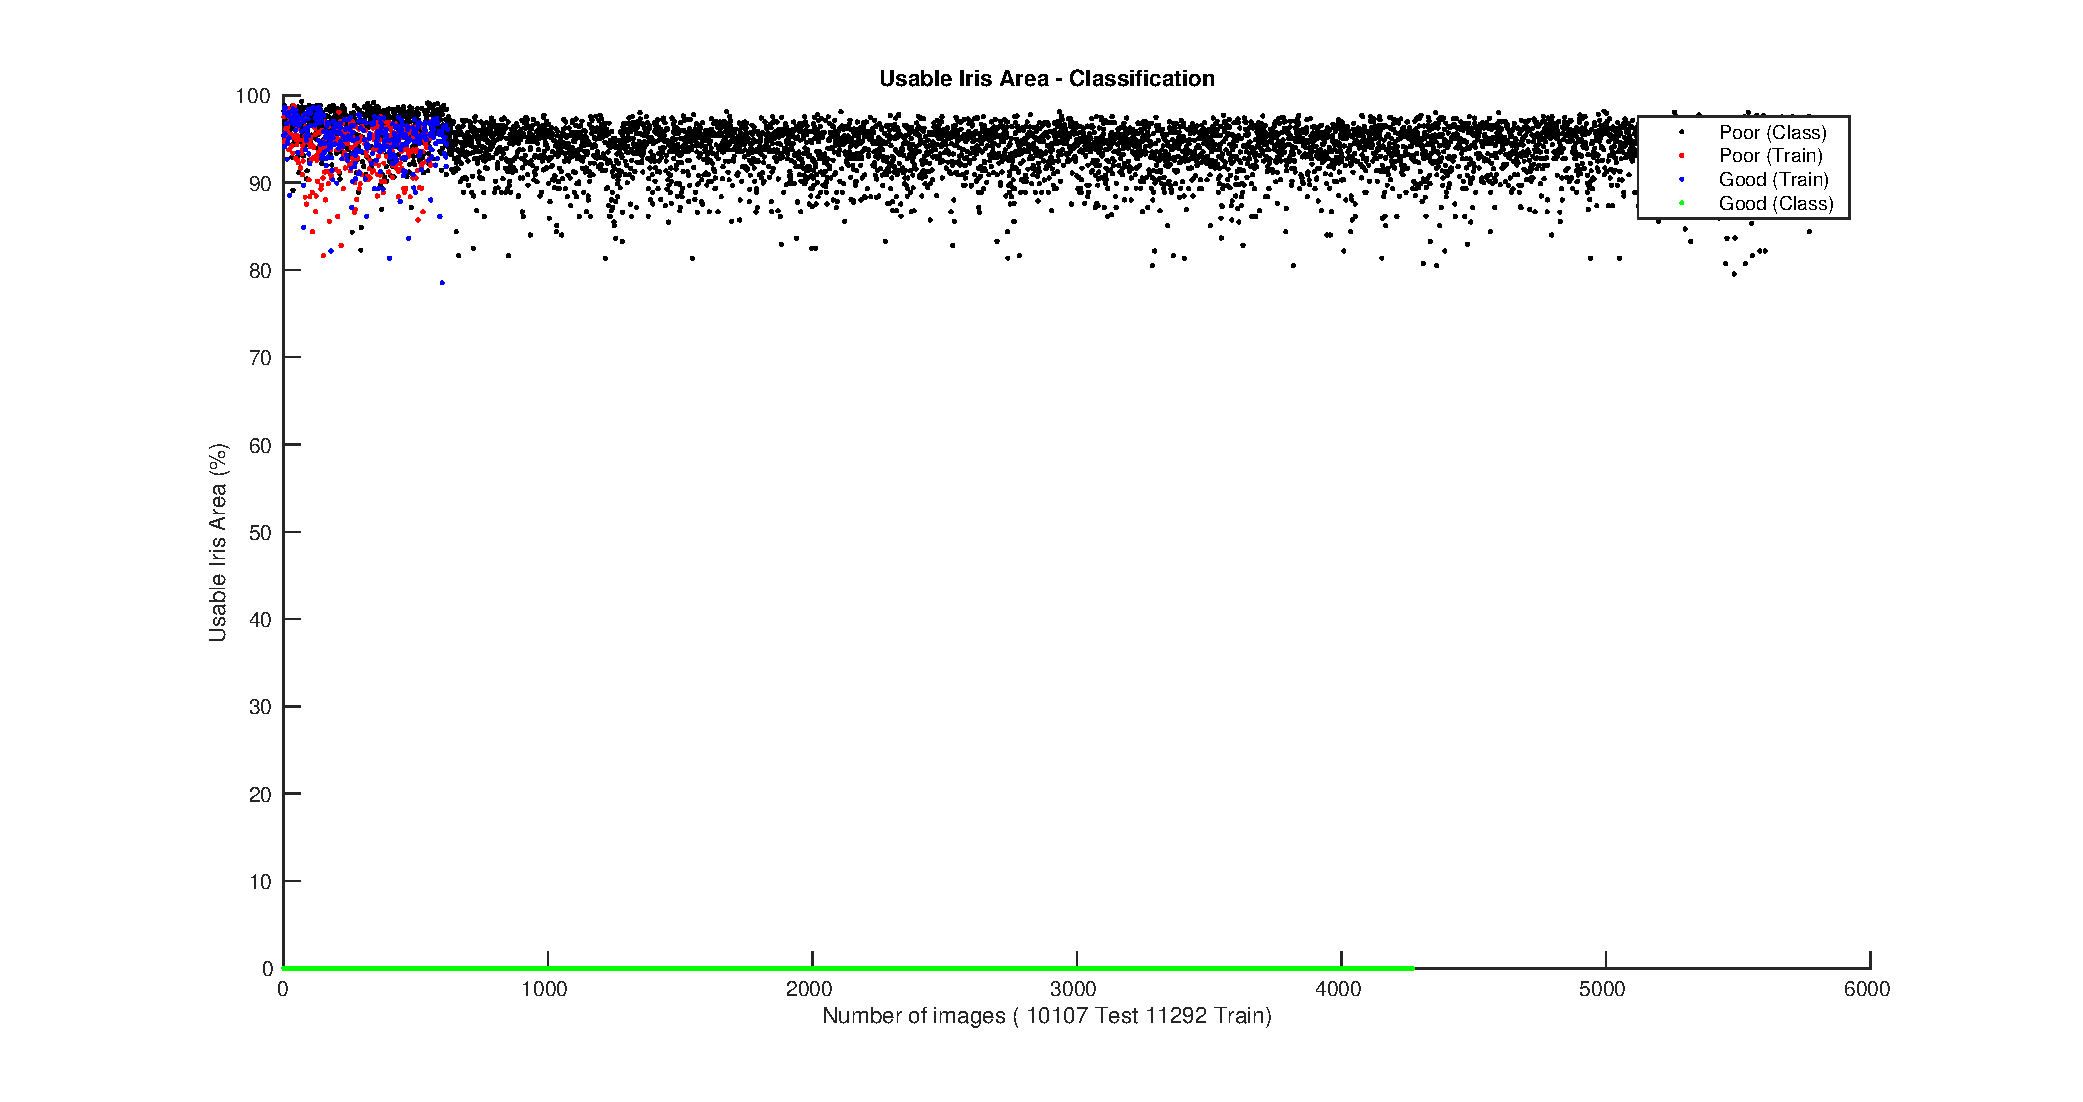
\includegraphics[width=0.9\linewidth, height=1.6cm]{pics/iqa_clas_usable_area}
		\caption{Res. of class. using BIQA UIA}
		\label{fig:clas_ua}
	\end{minipage}
	\begin{minipage}{0.48\linewidth}
		\centering
		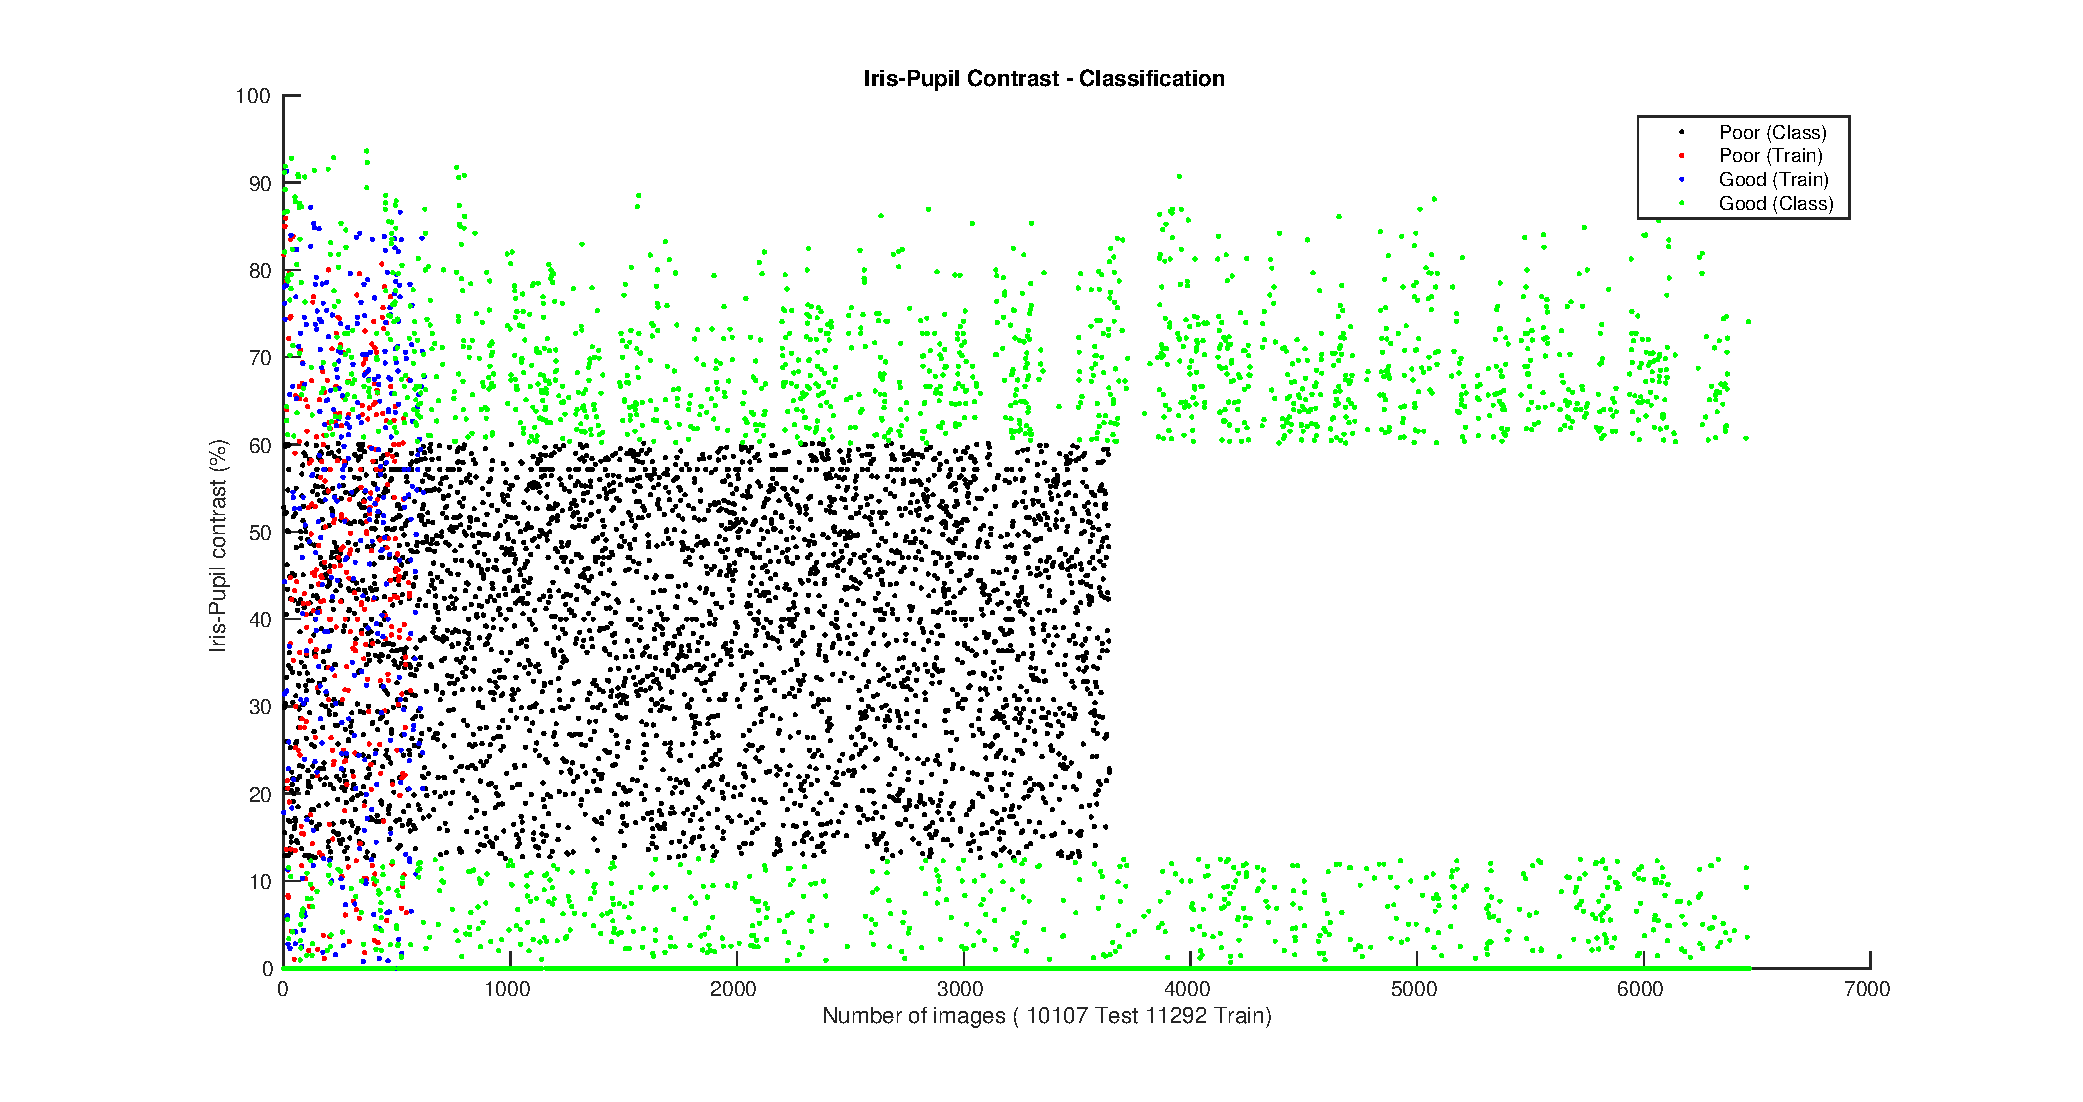
\includegraphics[width=0.9\linewidth, height=1.6cm]{pics/biqa_clas_ipc}
		\caption{Res. of class. using BIQA IPC}
		\label{fig:clas_ipc}
	\end{minipage}
	\hfill
	\begin{minipage}{0.48\linewidth}
		\centering
		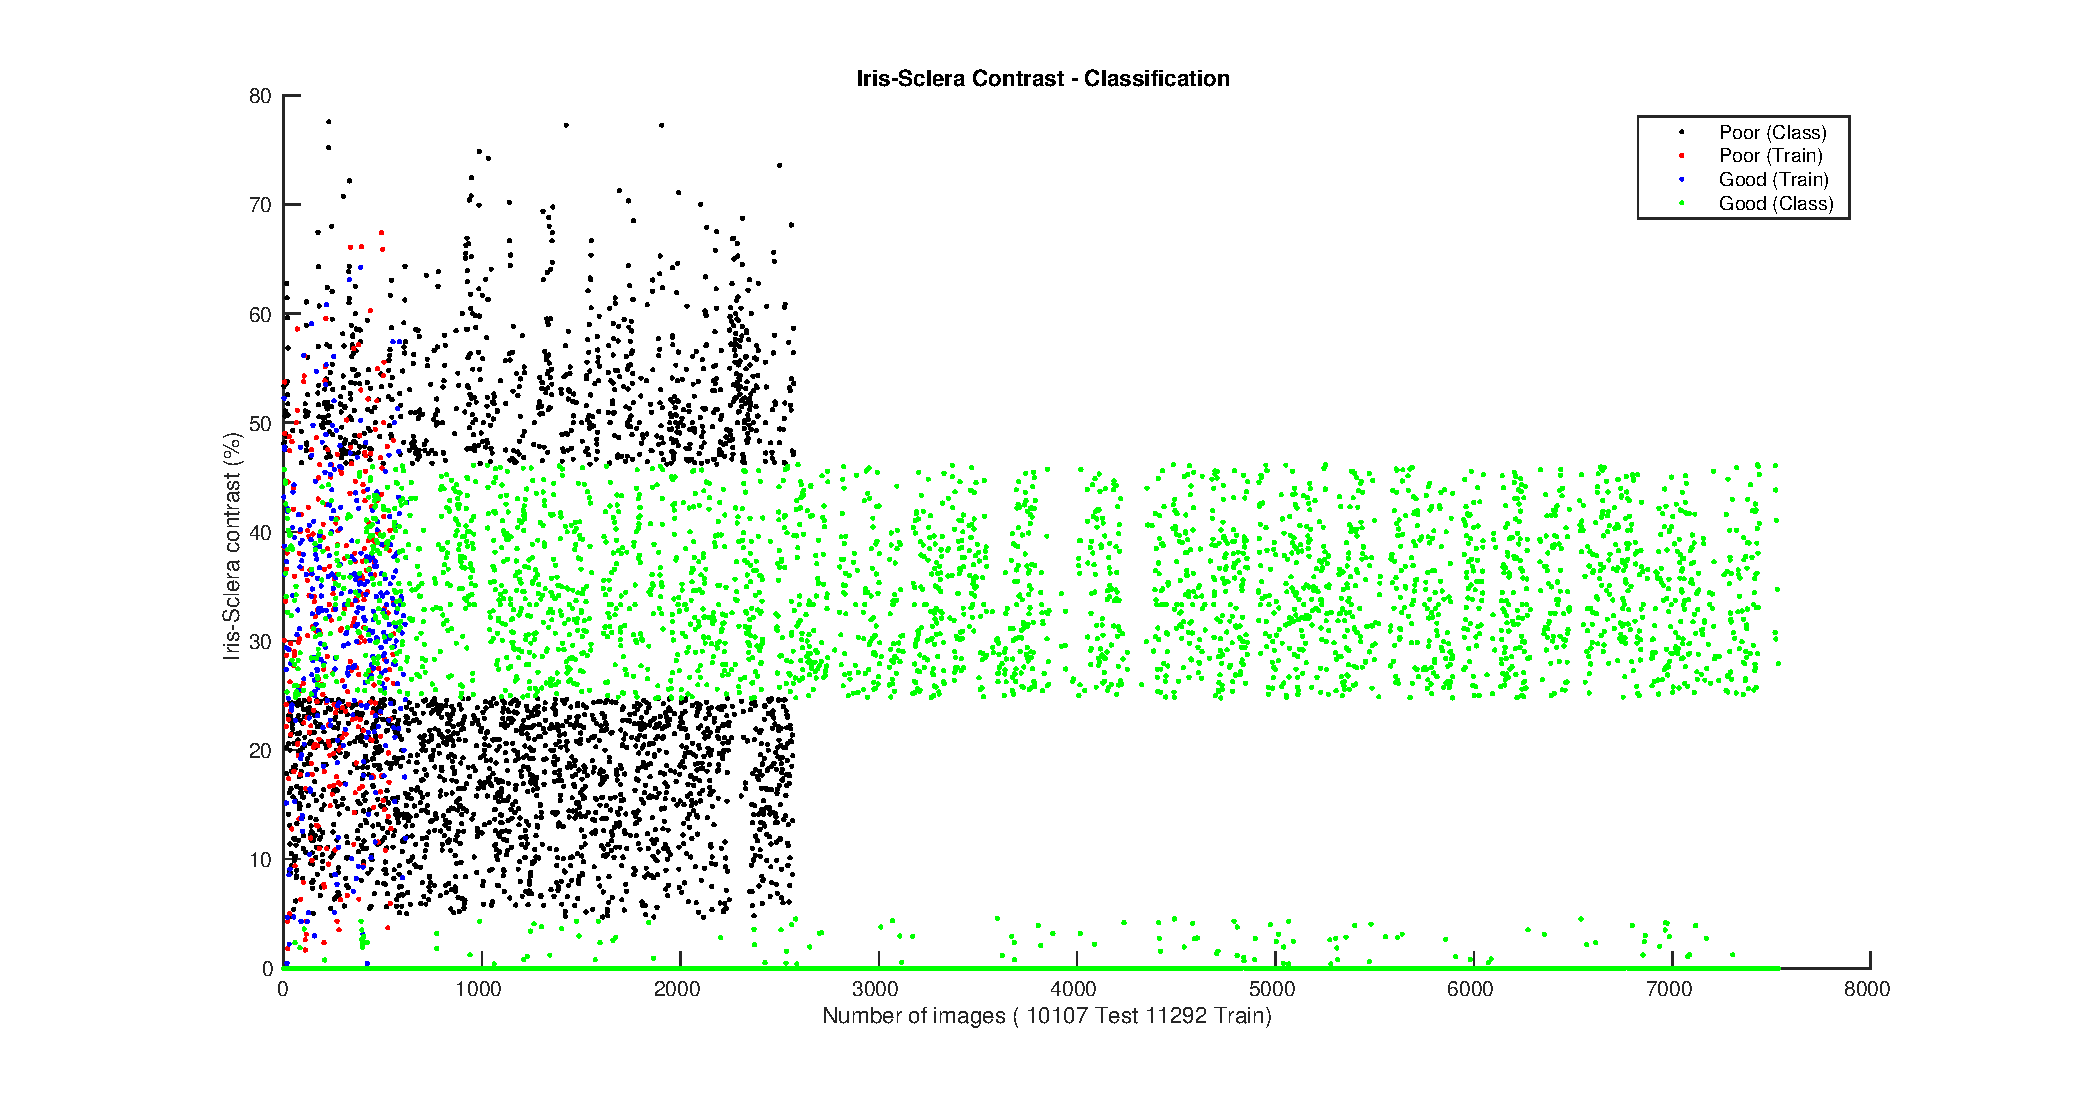
\includegraphics[width=0.9\linewidth, height=1.6cm]{pics/biqa_clas_isc}
		\caption{Res. of class. using BIQA ISC}
		\label{fig:clas_isc}
	\end{minipage}
	\begin{minipage}{0.48\linewidth}
		\centering
		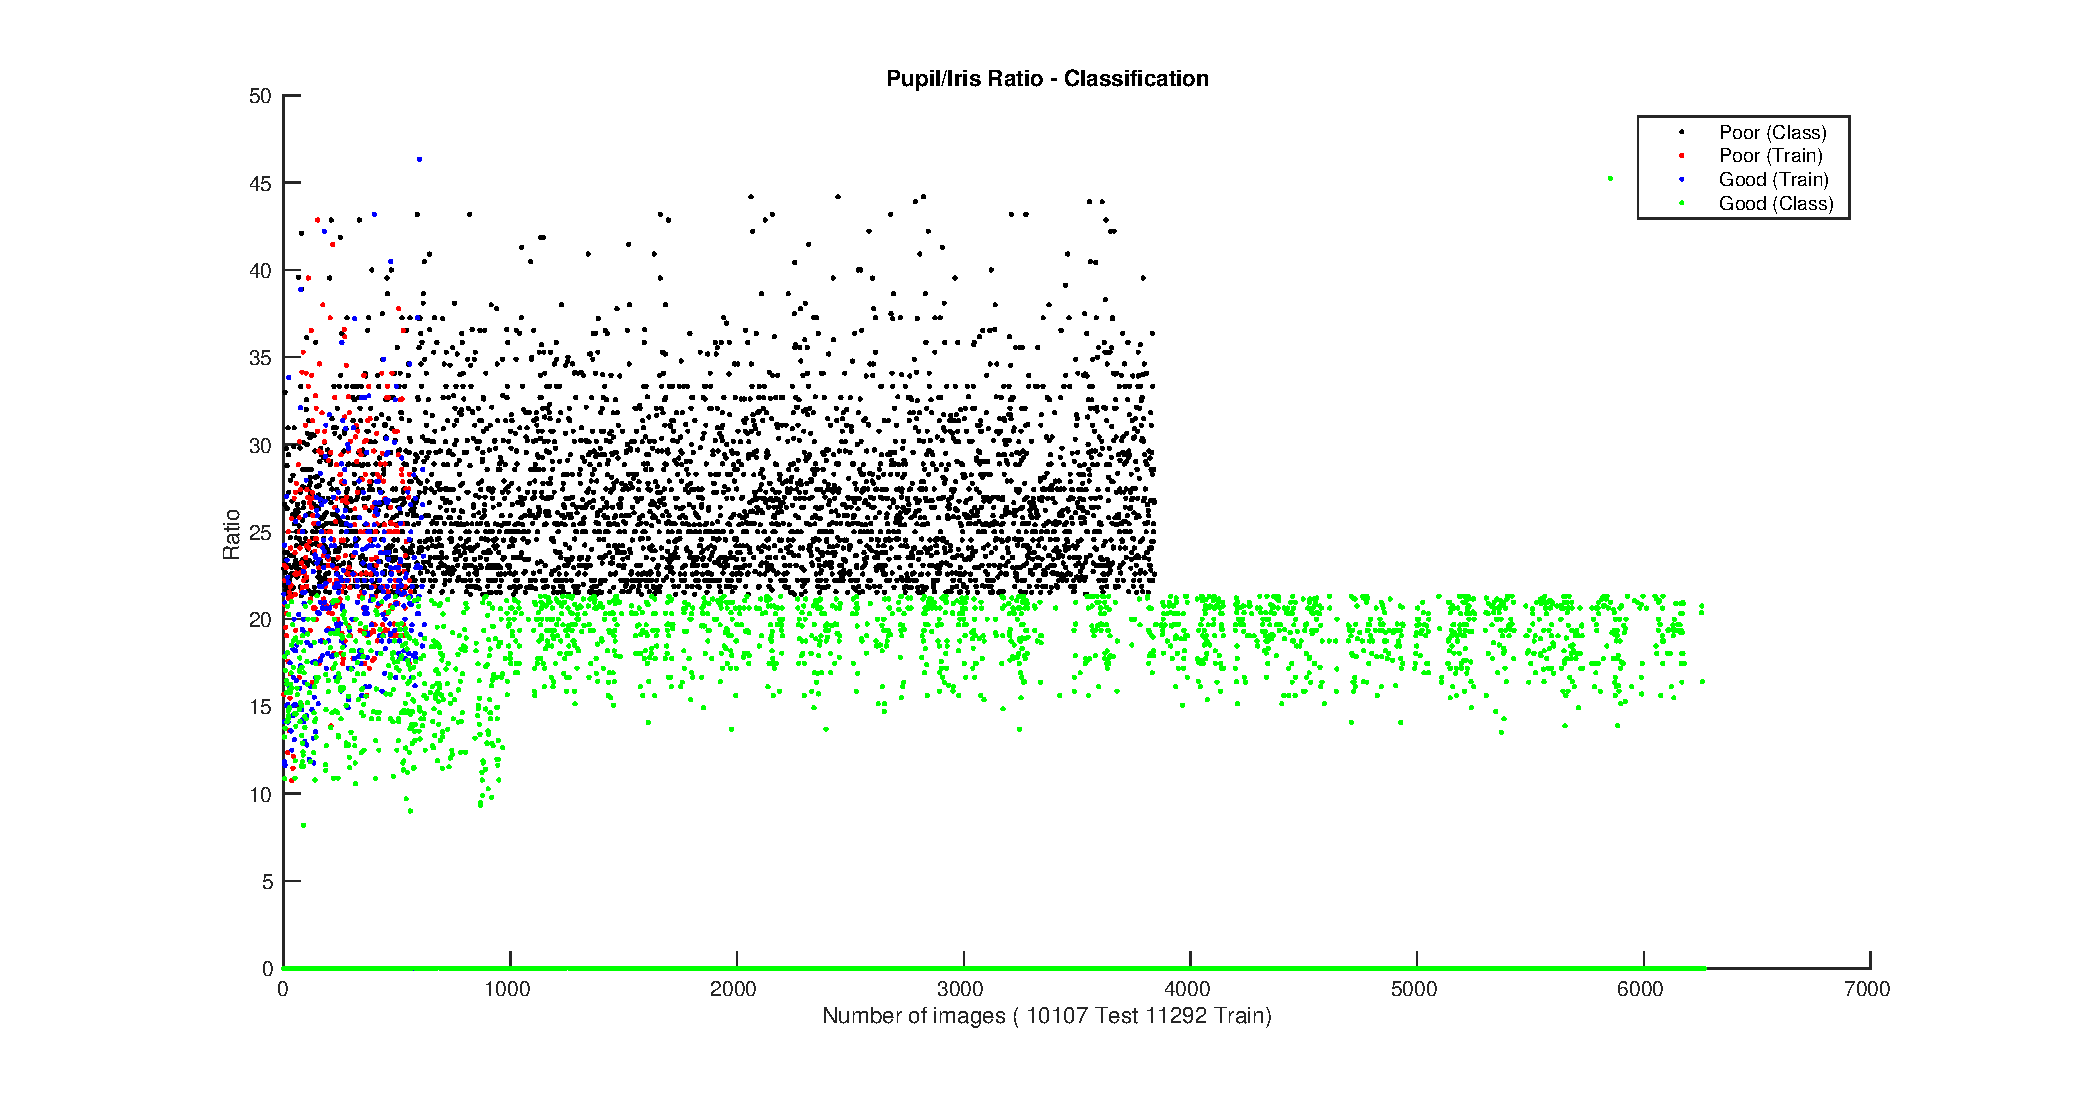
\includegraphics[width=0.9\linewidth, height=1.6cm]{pics/biqa_clas_pir}
		\caption{Res. of class. using BIQA pupil-iris rat.}
		\label{fig:clas_pir}
	\end{minipage}
	\hfill
	\begin{minipage}{0.48\linewidth}
		\centering
		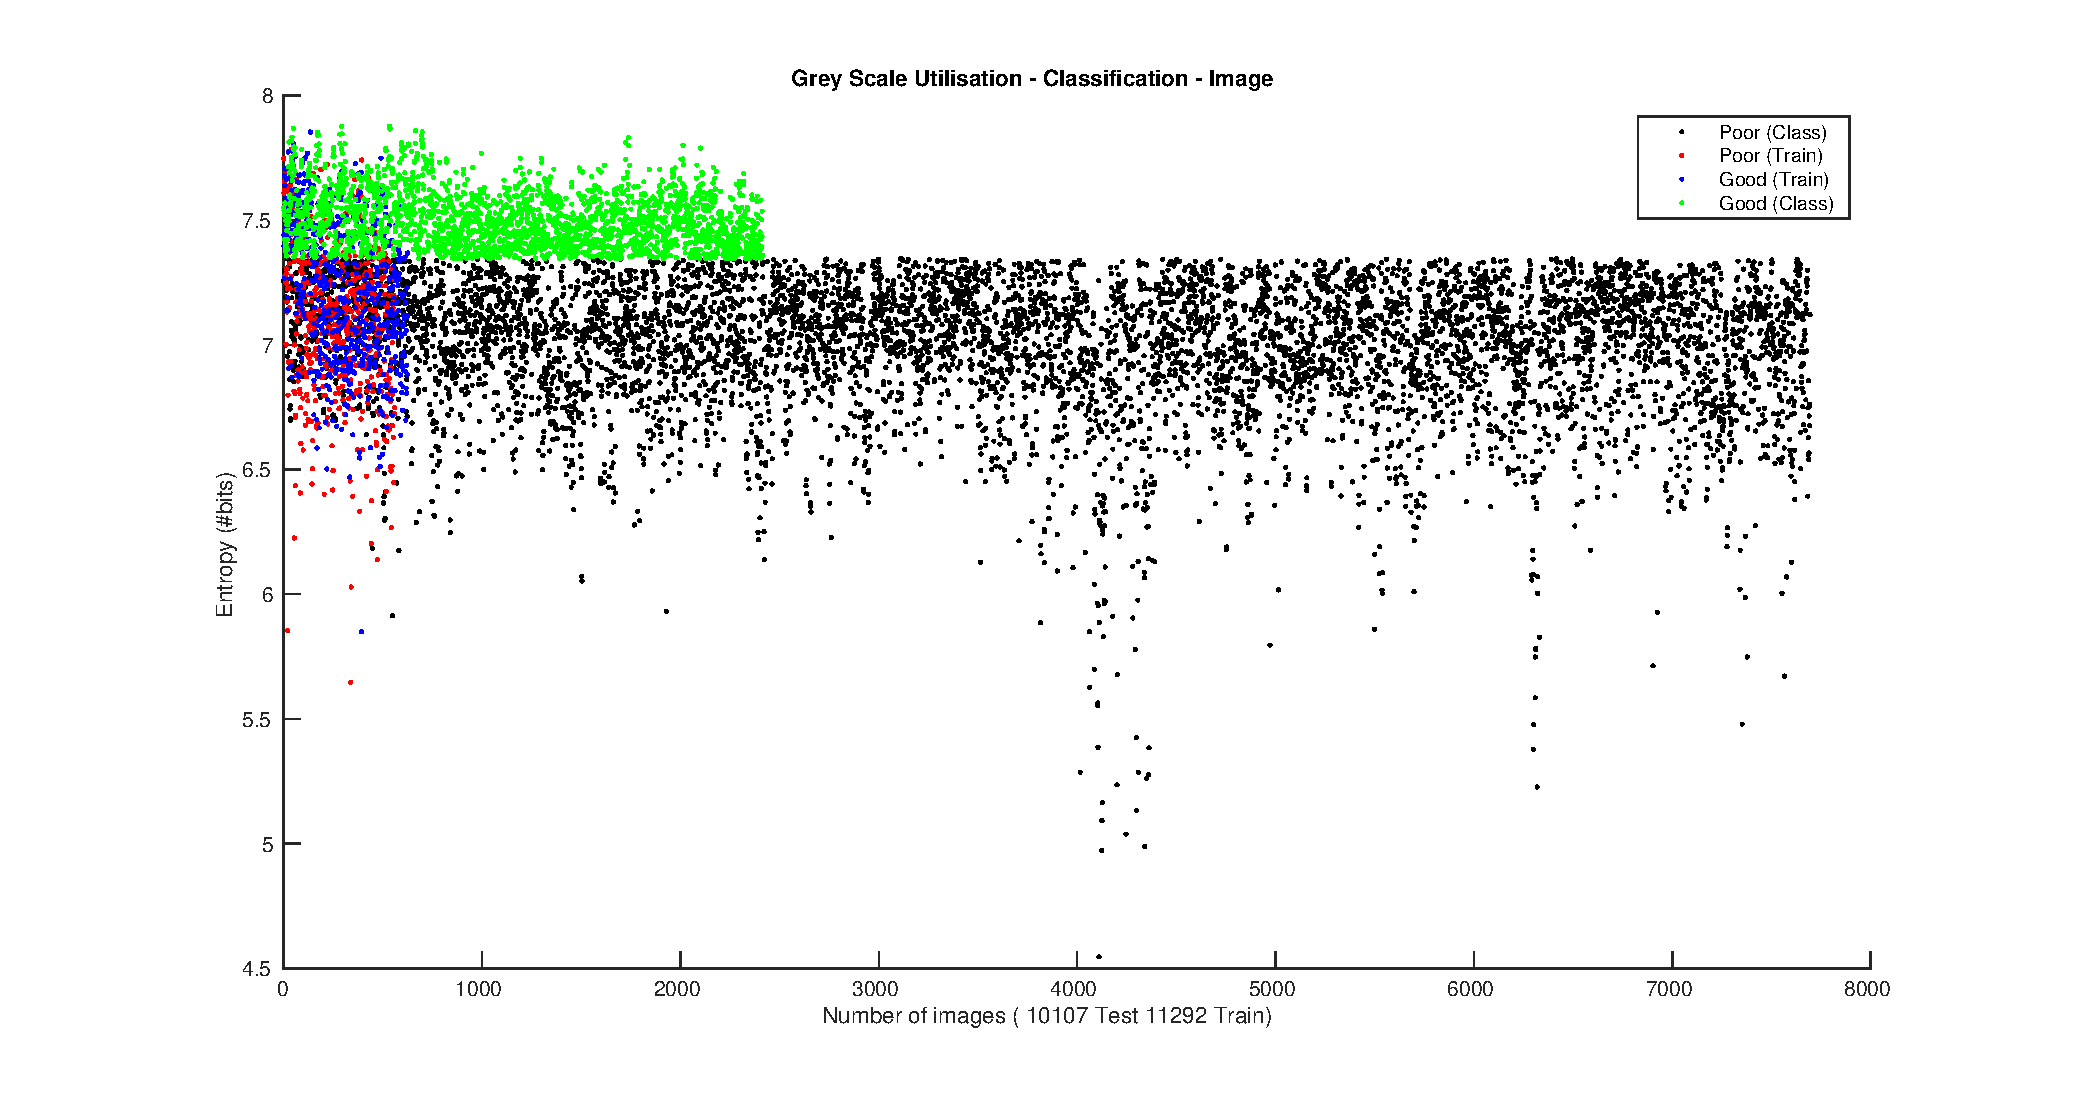
\includegraphics[width=0.9\linewidth, height=1.6cm]{pics/biqa_clas_gsu}
		\caption{Res. of class. using BIQA GSU}
		\label{fig:clas_gsu}
	\end{minipage}
	\begin{minipage}{0.48\linewidth}
		\centering
		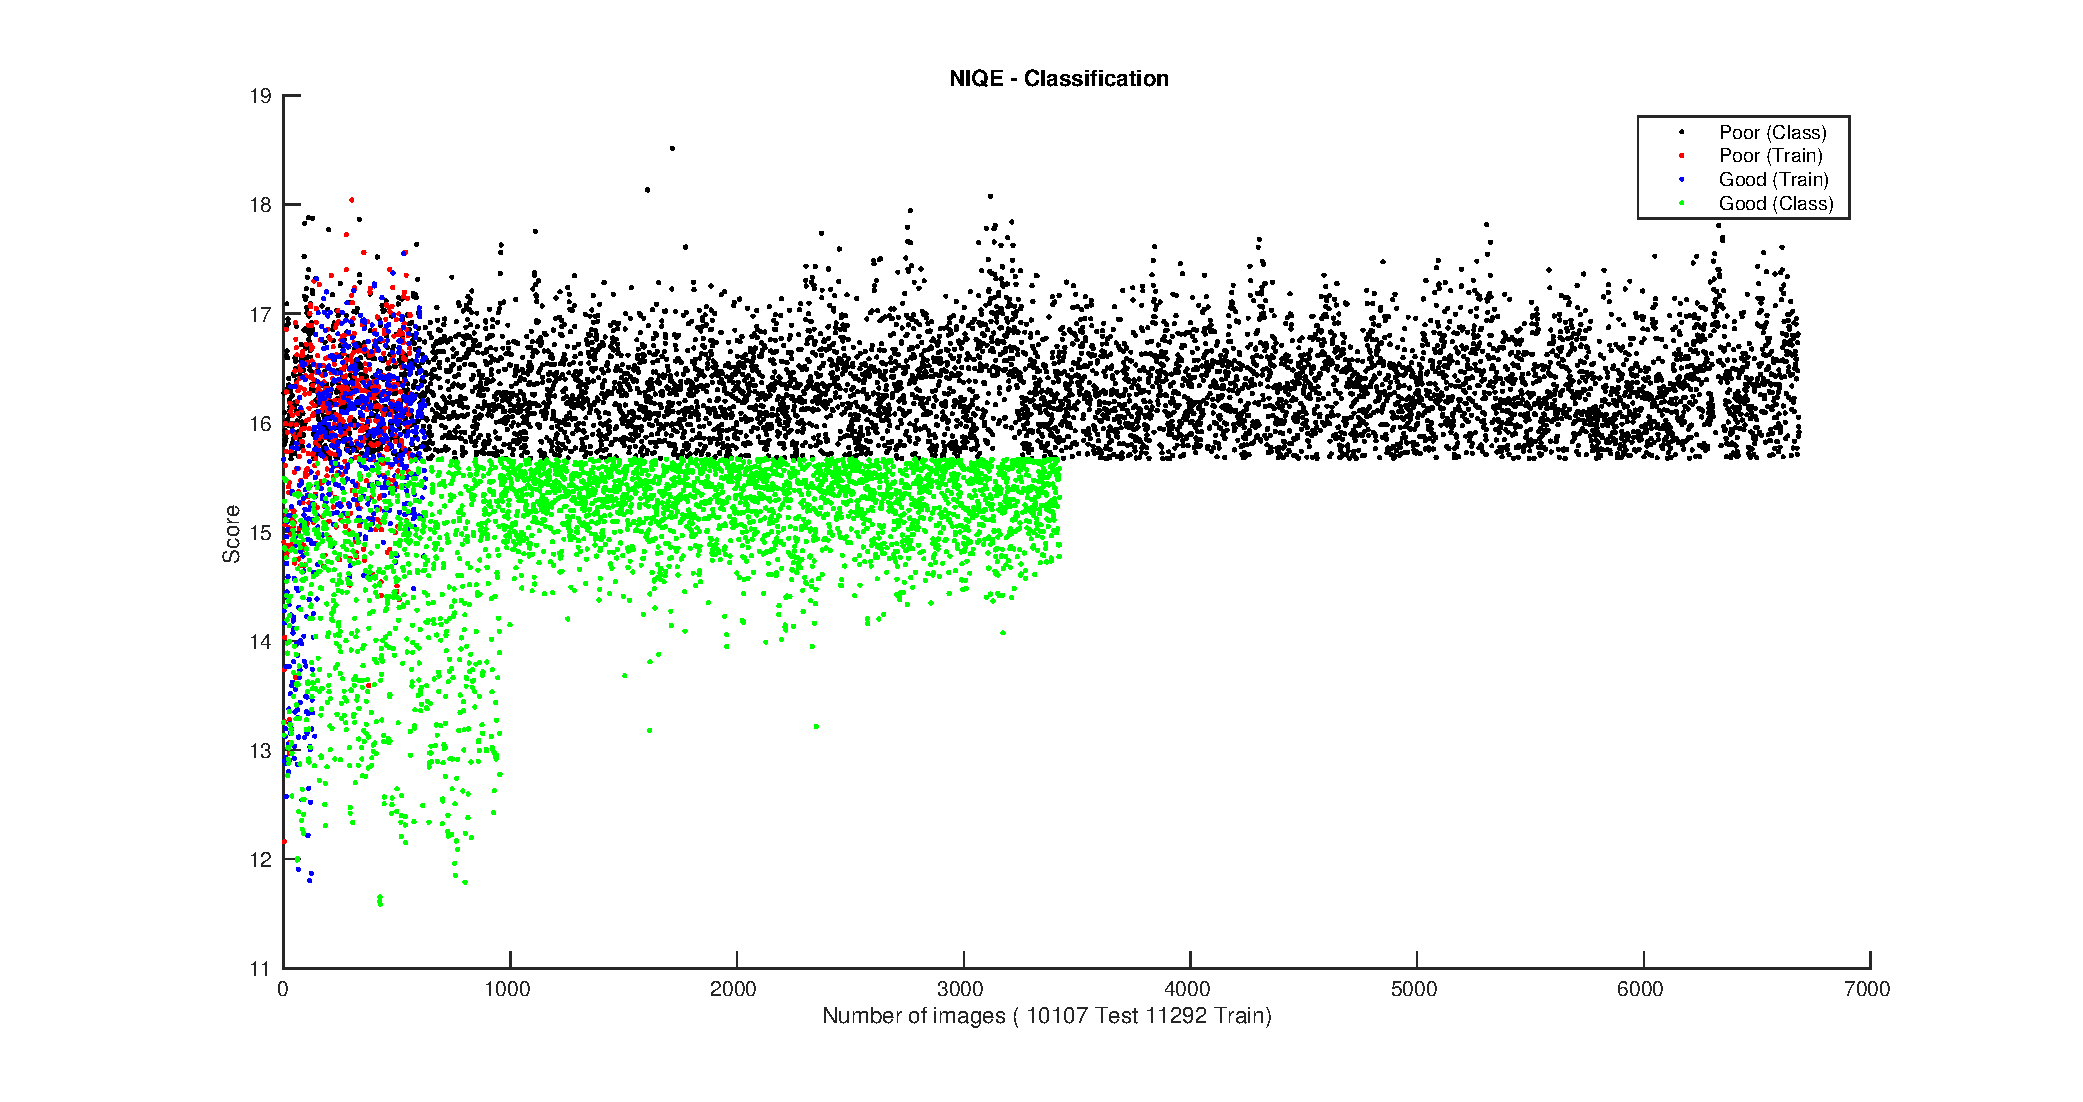
\includegraphics[width=0.9\linewidth, height=1.6cm]{pics/biqa_clas_niqe}
		\caption{Res. of class. using BIQA NIQE}
		\label{fig:clas_niqe}
	\end{minipage}
	\hfill
	\begin{minipage}{0.48\linewidth}
		\centering
		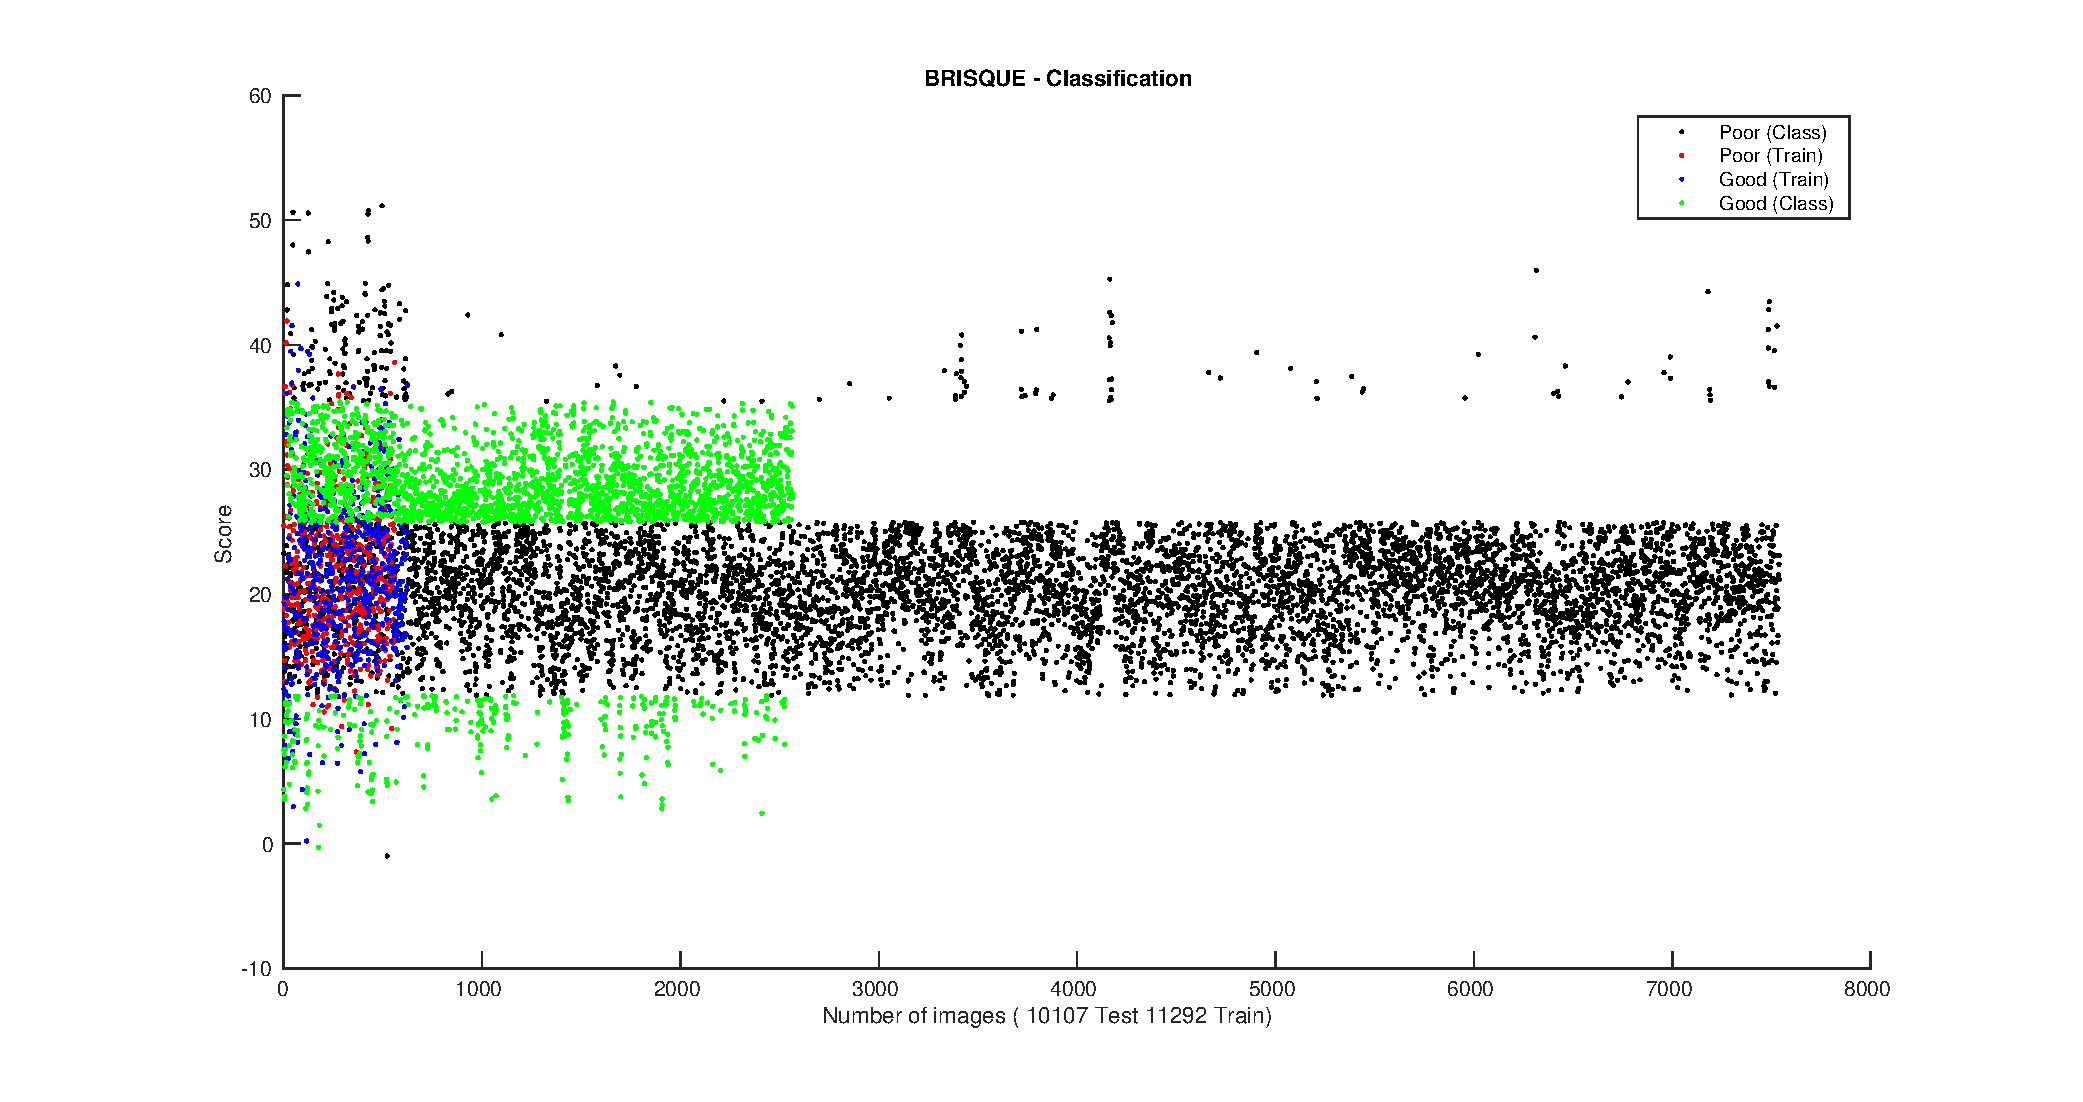
\includegraphics[width=0.9\linewidth, height=1.6cm]{pics/biqa_clas_brisque}
		\caption{Res. of class. using BIQA BRISQUE}
		\label{fig:clas_brisque}
	\end{minipage}
	\begin{minipage}{0.48\linewidth}
		\centering
		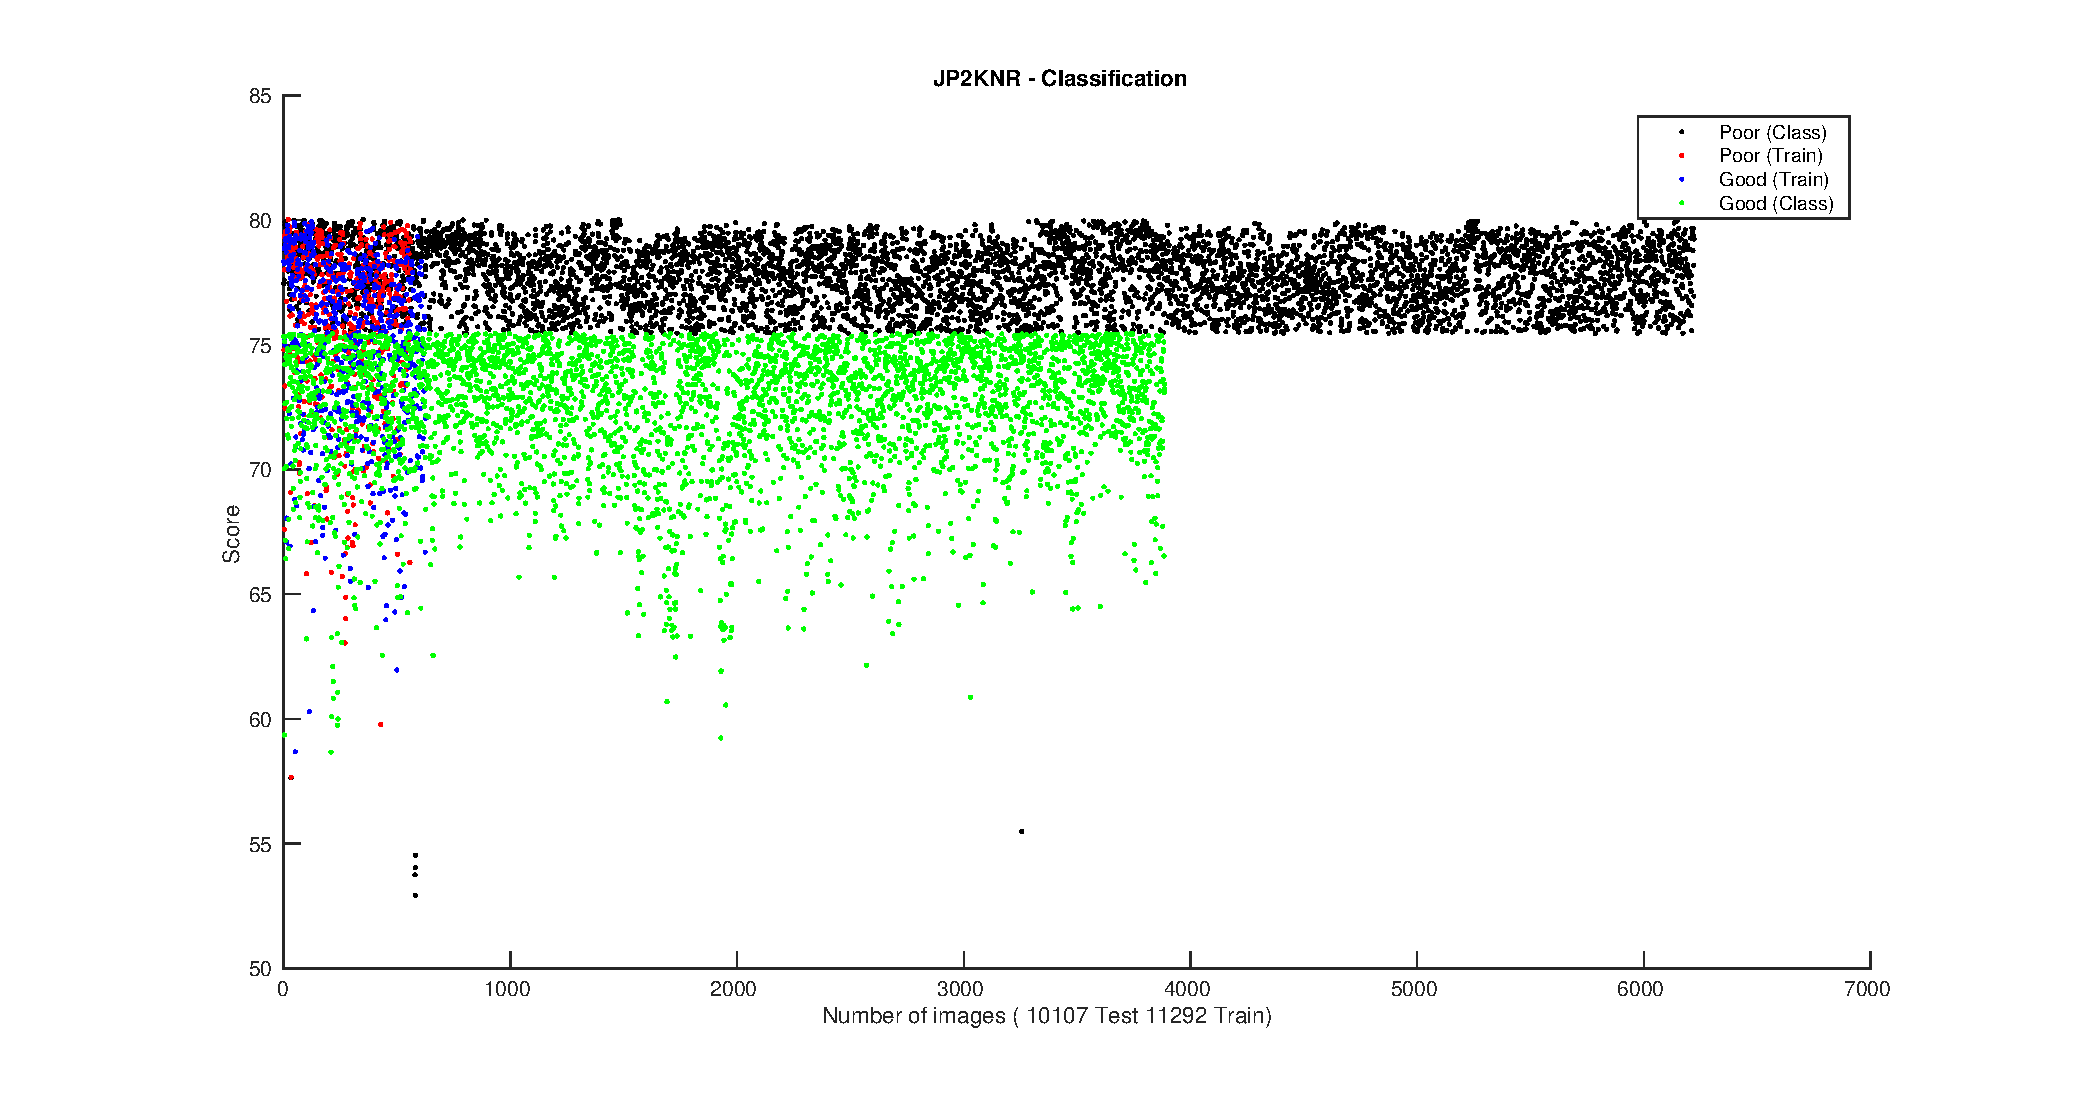
\includegraphics[width=0.9\linewidth, height=1.6cm]{pics/biqa_clas_jp2knr}
		\caption{Res. of class. using BIQA JP2KNR}
		\label{fig:clas_jp2knr}
	\end{minipage}
	\hfill
	\begin{minipage}{0.48\linewidth}
		\centering
		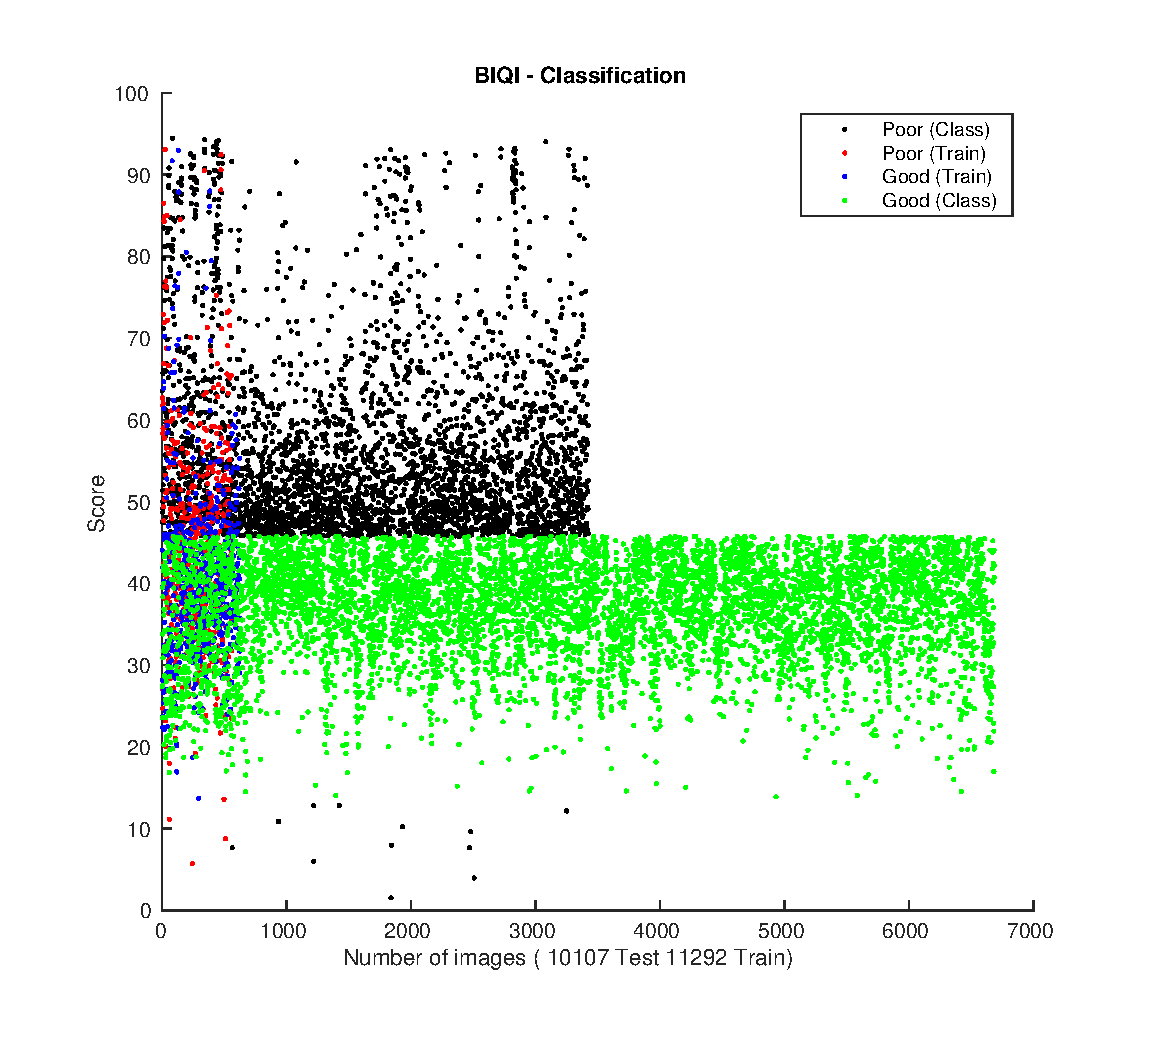
\includegraphics[width=0.9\linewidth, height=1.6cm]{pics/biqa_clas_biqi}
		\caption{Res. of class. using BIQA BIQI}
		\label{fig:clas_biqi}
	\end{minipage}
\end{figure}

